\section{Results}
\label{sec:results}

\subsection{Descriptive Speed Behavior Characterization}
\label{sec:res_descriptive}

Figure~\ref{fig:speed_by_mode} presents the distribution of trip-level mean and maximum speeds by operating mode. The three scooter operating modes produce dramatically different speed profiles. In TUB (turbo) mode, the mean trip speed is 16.7~km/h and the mean maximum speed is 25.0~km/h---just at the Korean regulatory threshold. In STD (standard) mode, these values drop to 14.2~km/h and 20.8~km/h, while ECO mode further reduces them to 11.0~km/h and 16.3~km/h. The speeding rate---defined as the fraction of trips in which the maximum speed exceeds 25~km/h---exhibits a corresponding gradient: 54.0\% for TUB, 0.93\% for STD, and 1.1\% for ECO mode. The near-equivalence of STD and ECO speeding rates (both approximately 1\%) contrasts sharply with the 54-fold higher rate in TUB mode, confirming that the speed governor is the dominant determinant of speeding behavior.

Overall, 29.6\% of all valid trips contain at least one speed reading exceeding 25~km/h. At the user level, 60.9\% of users never exceed this threshold during any of their recorded trips, 21.8\% speed on fewer than half of their trips, and 17.3\% speed on more than half. This concentration of speeding among a minority of frequent speeders motivates our rider typology analysis (Section~\ref{sec:res_typology}).

\begin{figure}[htbp]
\centering
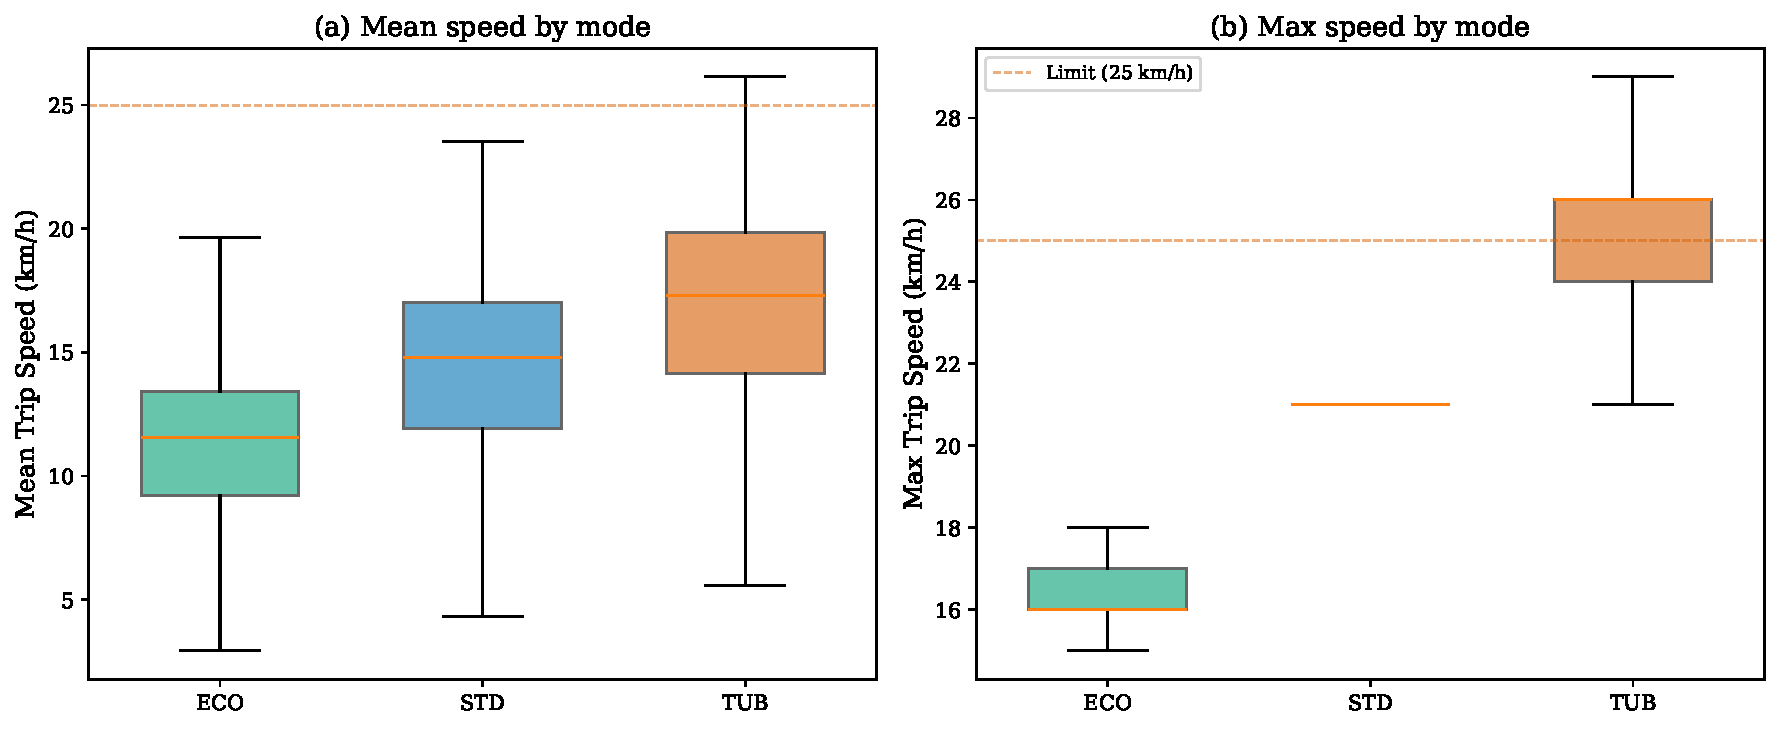
\includegraphics[width=\textwidth]{figures/fig4_speed_by_mode.pdf}
\caption{Distributions of trip-level mean speed and maximum speed by operating mode (ECO, STD, TUB). Box plots show median, interquartile range, and 5th/95th percentiles. The dashed horizontal line indicates the 25~km/h regulatory speed limit.}
\label{fig:speed_by_mode}
\end{figure}

Figure~\ref{fig:temporal} shows temporal patterns of trip volume and speeding. The daily distribution is bimodal, with peaks during the morning commute (8--9~AM) and evening (6--10~PM). Speeding rates are slightly elevated during late-night hours (11~PM--2~AM) and on weekends, likely reflecting reduced traffic congestion and lower perceived enforcement risk. The hour-by-day-of-week speeding heatmap (Figure~\ref{fig:heatmap}) reveals that weekend evenings (Friday--Sunday, 8~PM--midnight) exhibit the highest sustained speeding rates.

Provincial variation in speeding is substantial. Chungnam province has the highest speeding rate (45.8\%), followed by Gyeongbuk (42.6\%) and Gangwon (41.7\%), while Ulsan has the lowest (17.6\%). This variation partly reflects differences in operating mode composition---provinces where TUB mode is more prevalent naturally exhibit higher speeding rates---but city-specific models (Section~\ref{sec:res_robust}) confirm that geographic differences persist after controlling for mode.

\begin{figure}[htbp]
\centering
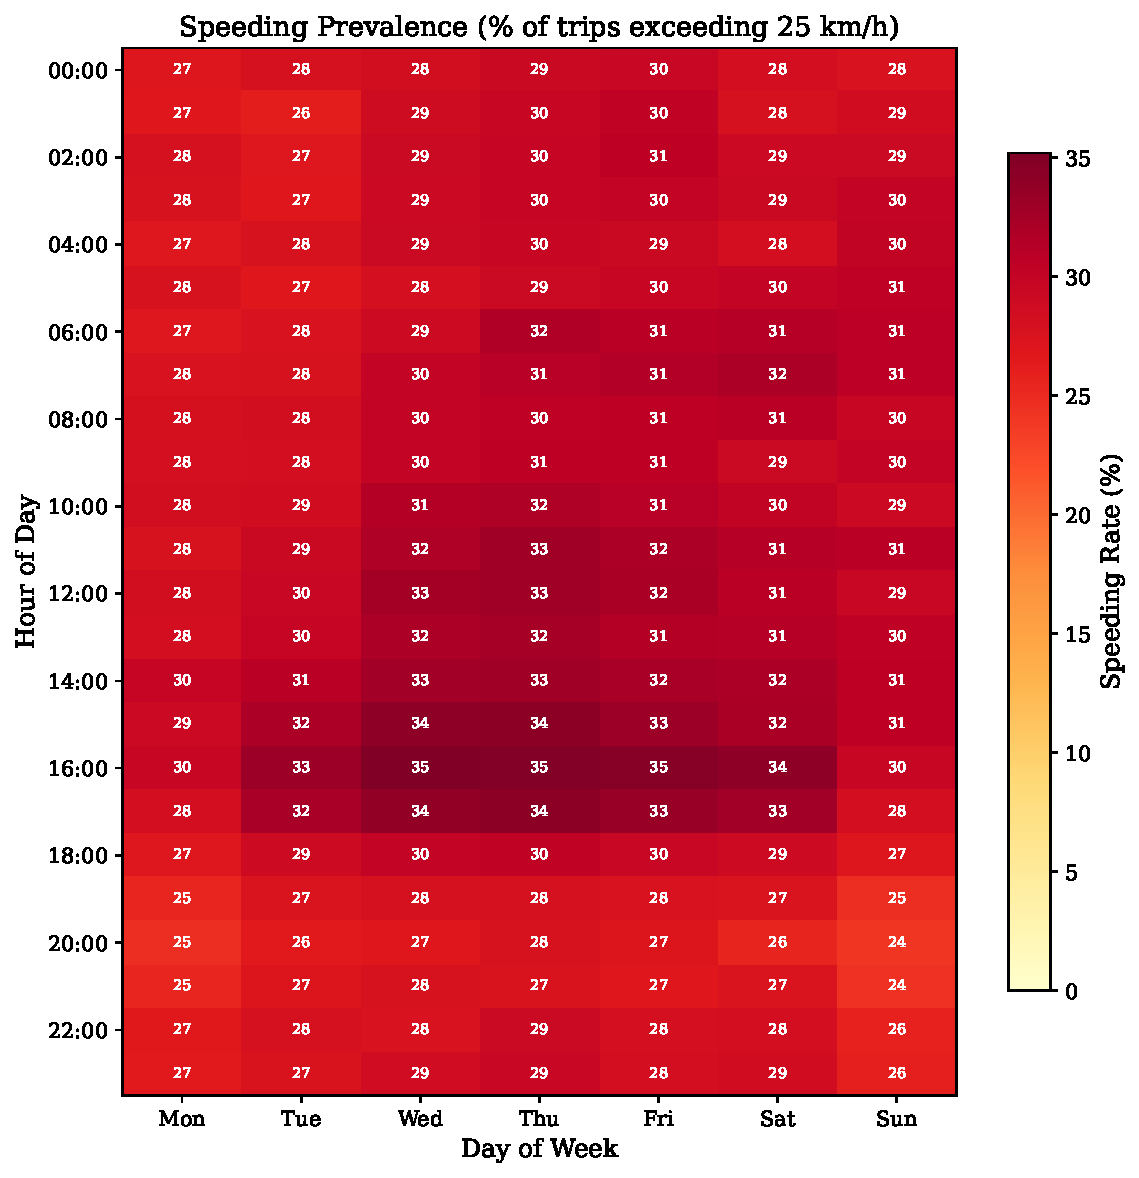
\includegraphics[width=\textwidth]{figures/fig5_speeding_heatmap.pdf}
\caption{Speeding prevalence heatmap by hour of day (rows) and day of week (columns). Color intensity indicates the percentage of trips with maximum speed exceeding 25~km/h.}
\label{fig:heatmap}
\end{figure}

\subsection{Spatial Patterns of Speed Behavior}
\label{sec:res_spatial}

\subsubsection{Global Spatial Autocorrelation}

Table~\ref{tab:morans} reports global Moran's $I$ values for hex-level speeding rates in five major cities (see also Figure~\ref{fig:morans_comparison}, Appendix). All values are positive and highly significant ($p < 0.001$), confirming that speeding is spatially clustered rather than randomly distributed. Daegu exhibits the strongest spatial autocorrelation ($I = 0.712$, $z = 24.5$), reflecting its compact urban structure with sharply distinct high- and low-speeding neighborhoods. Seoul shows moderate autocorrelation ($I = 0.213$, $z = 10.3$), consistent with its more heterogeneous and polycentric urban form.

\begin{table}[htbp]
\centering
\caption{Global Moran's $I$ for hex-level speeding rates by city.}
\label{tab:morans}
\small
\begin{tabular}{lrrrl}
\toprule
\textbf{City} & \textbf{Hex cells} & \textbf{Moran's $I$} & \textbf{$z$-score} & \textbf{$p$-value} \\
\midrule
Seoul & 531 & 0.213 & 10.3 & $< 0.001$ \\
Daejeon & 248 & 0.235 & 8.1 & $< 0.001$ \\
Suwon & 197 & 0.156 & 5.9 & $< 0.001$ \\
Busan & 311 & 0.301 & 11.4 & $< 0.001$ \\
Daegu & 268 & 0.712 & 24.5 & $< 0.001$ \\
\bottomrule
\end{tabular}
\end{table}

\subsubsection{Hotspot Detection}

Figure~\ref{fig:seoul_hotspot} presents the four-panel spatial analysis for Seoul: trip density, mean speeding rate, Getis-Ord $G_i^*$ hotspots, and LISA clusters. Figure~\ref{fig:daejeon_hotspot} shows the corresponding analysis for Daejeon. Of Seoul's 531 hex cells, 101 (19\%) are identified as statistically significant hot spots (high speeding clusters) and 123 (23\%) as cold spots (low speeding clusters); the remaining 307 cells (58\%) are not statistically significant. Hot spots concentrate in southern Seoul (Gangnam, Seocho, Songpa districts), while cold spots are more prevalent in central and northern areas. LISA analysis identifies 46 High-High (HH) clusters and 70 Low-Low (LL) clusters, with relatively few spatial outliers (HL: 15, LH: 22).

The infrastructure overlay analysis (Section~\ref{sec:meth_spatial}) reveals a noteworthy pattern (see also Figure~\ref{fig:hotspot_infra}, Appendix). Hot-spot and cold-spot hexes have similar fractions of major roads (0.210 vs.\ 0.207), suggesting that road hierarchy alone does not explain spatial variation in speeding. However, cold spots have more than twice the cycling infrastructure coverage of hot spots (0.033 vs.\ 0.015), providing suggestive evidence that dedicated cycling infrastructure may be associated with lower speeding rates---a finding we explore further in the hurdle model (Section~\ref{sec:res_hurdle}). Corridor-level maps for Gangnam, Hongdae, and Yeouido are provided in Figure~\ref{fig:corridor} (Appendix).

\begin{figure}[htbp]
\centering
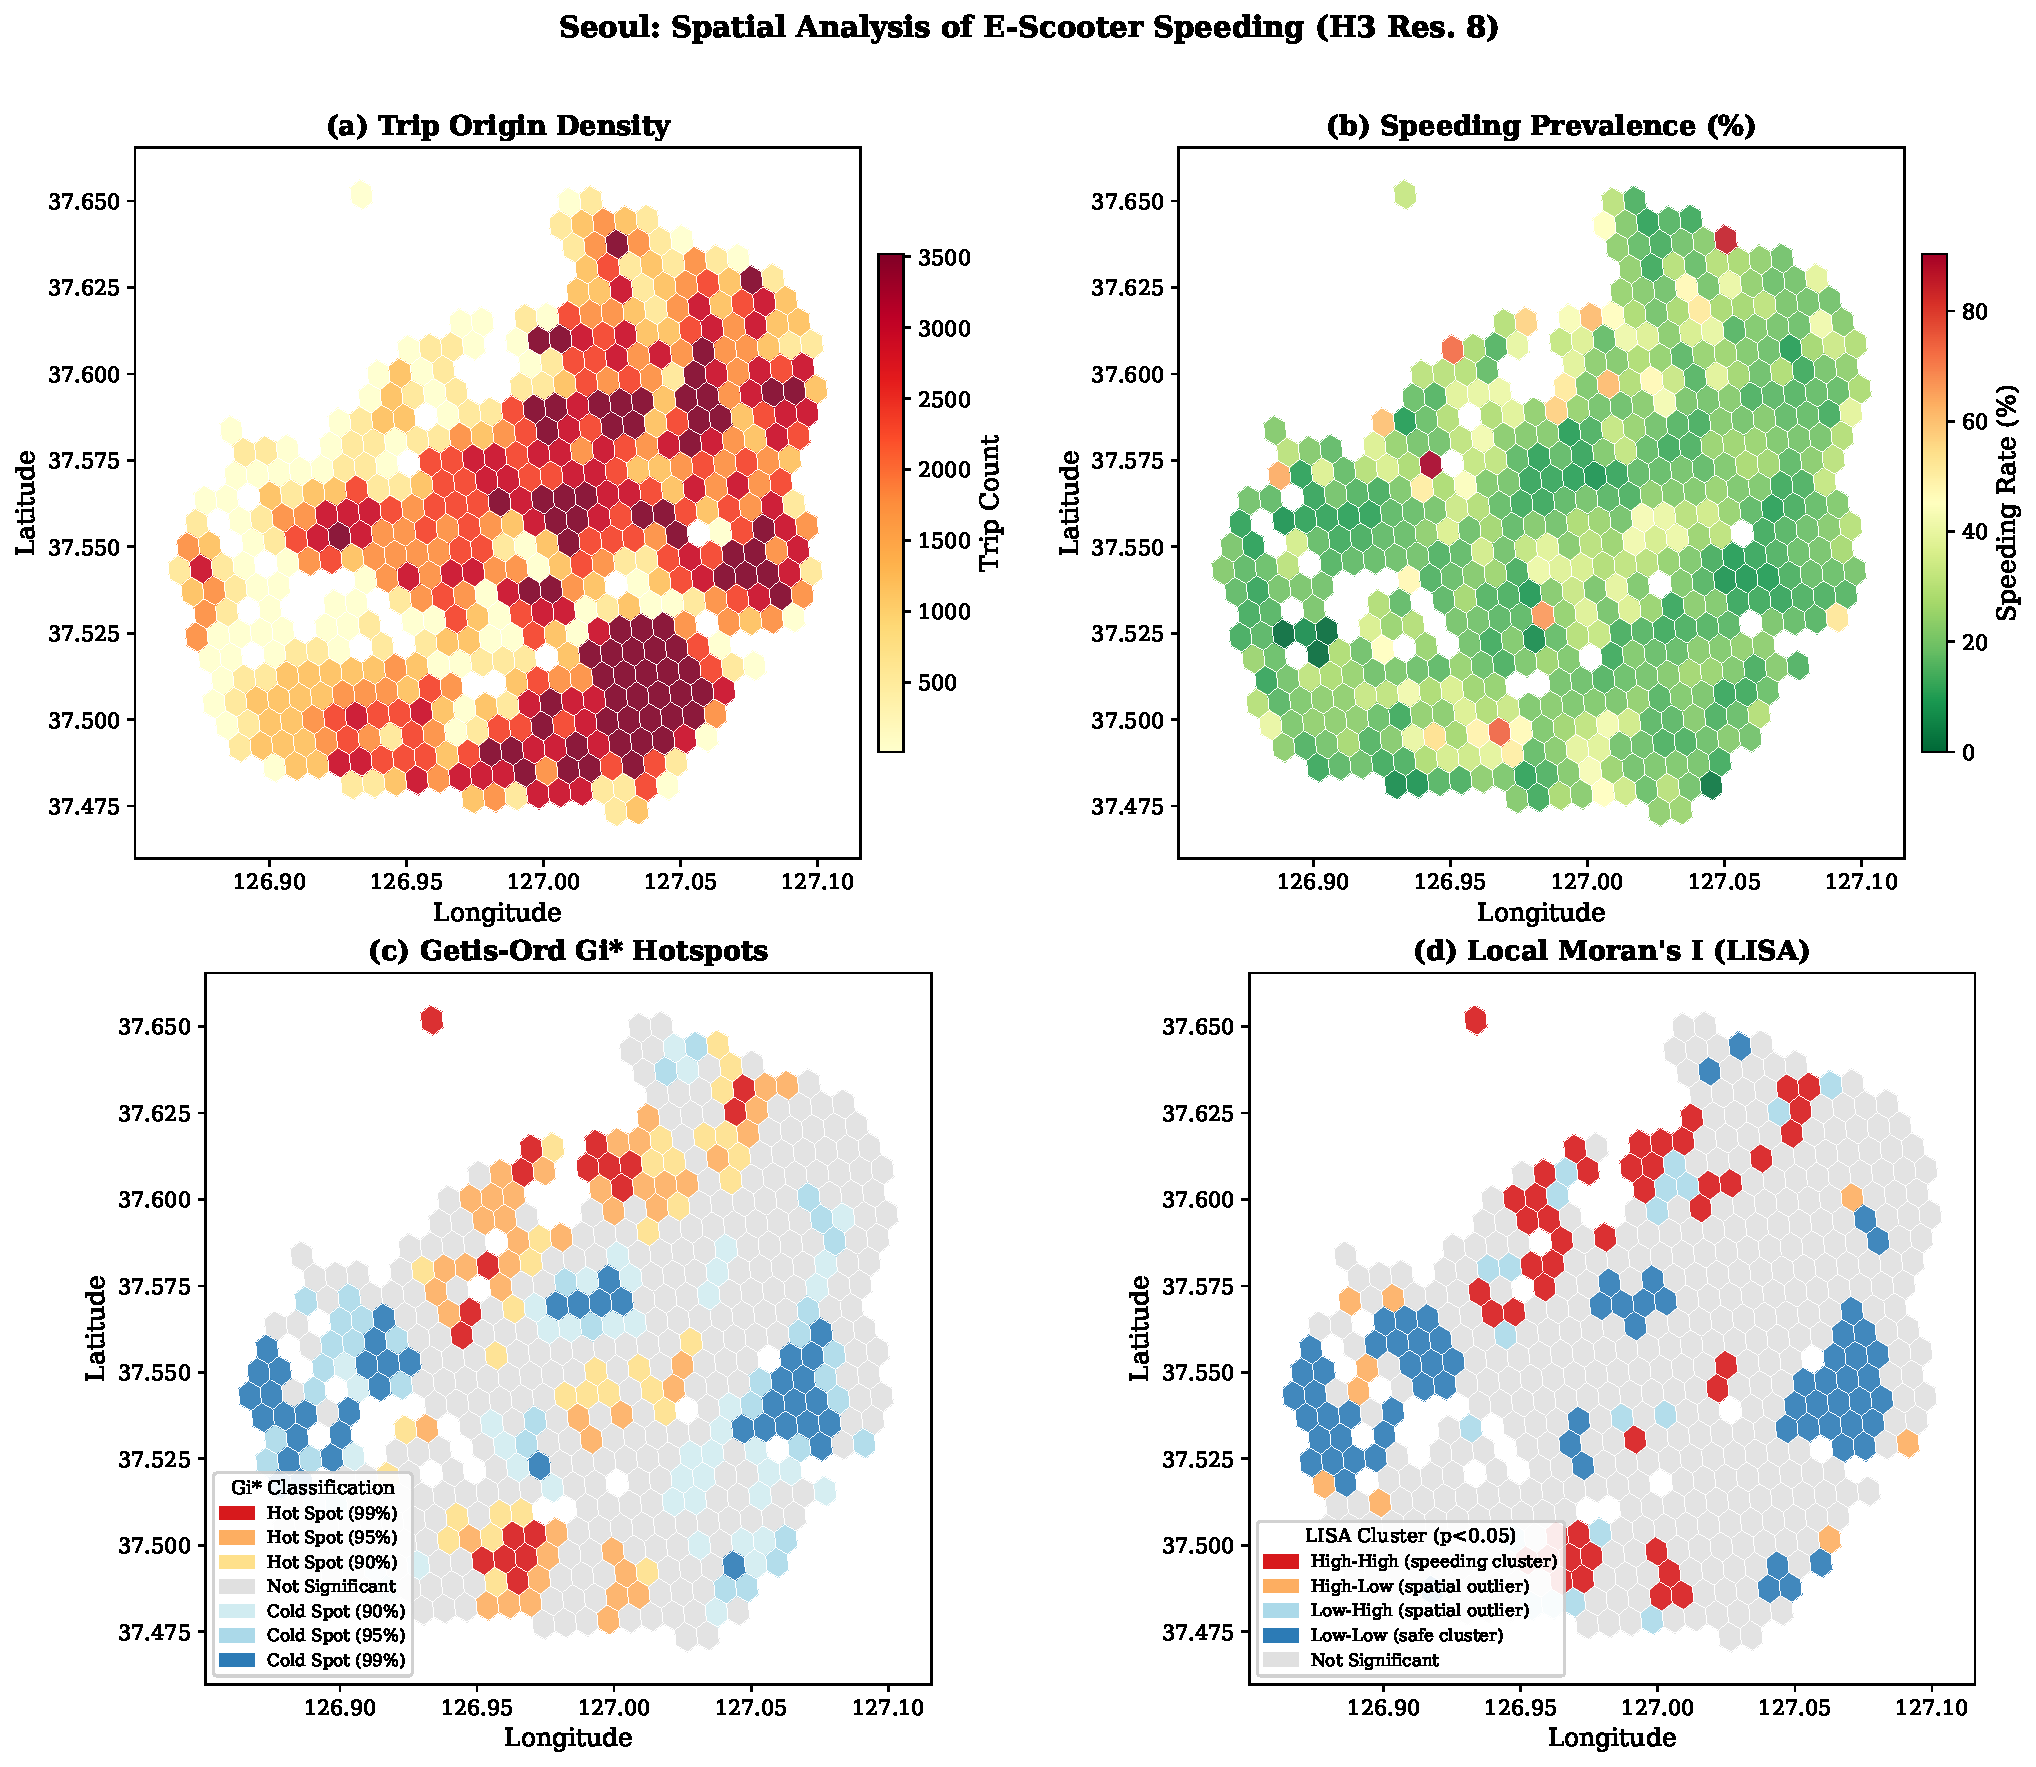
\includegraphics[width=\textwidth]{figures/fig6_seoul_hotspot.pdf}
\caption{Spatial analysis of speed behavior in Seoul using H3 hexagonal grid (resolution 8). Four panels: (a) trip density, (b) mean speeding rate, (c) Getis-Ord $G_i^*$ hot spots and cold spots, and (d) LISA cluster classification (HH, LL, HL, LH).}
\label{fig:seoul_hotspot}
\end{figure}

\begin{figure}[htbp]
\centering
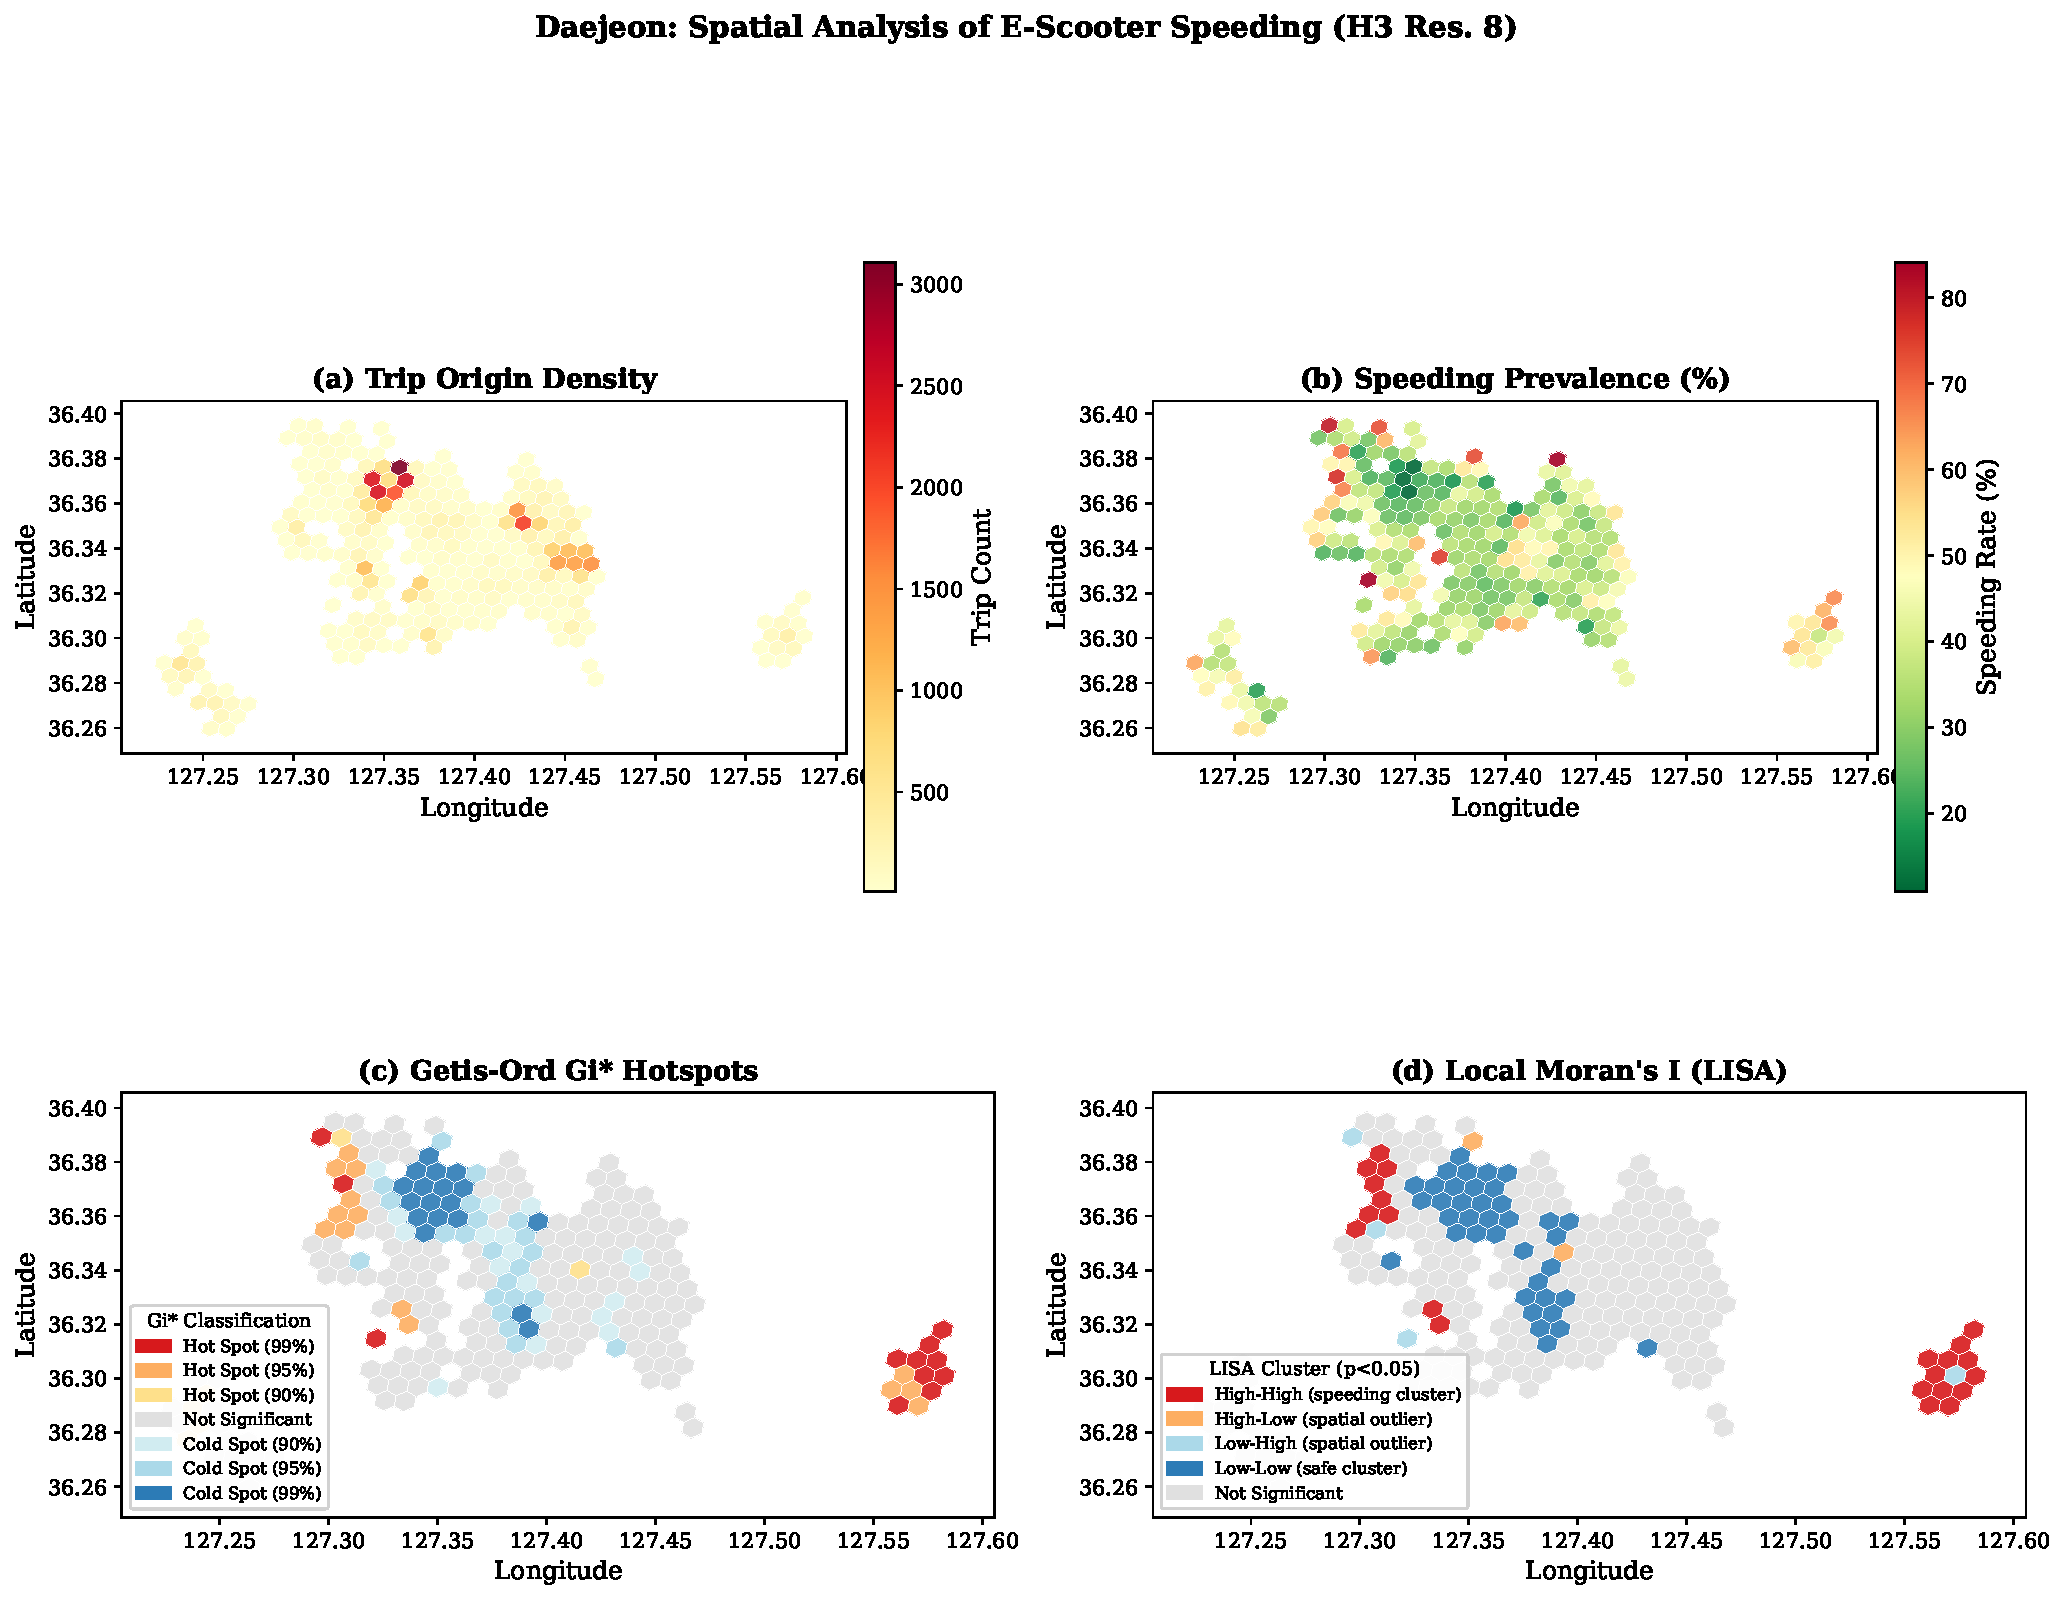
\includegraphics[width=\textwidth]{figures/fig7_daejeon_hotspot.pdf}
\caption{Spatial analysis of speed behavior in Daejeon, following the same four-panel layout as Figure~\ref{fig:seoul_hotspot}.}
\label{fig:daejeon_hotspot}
\end{figure}

\subsection{Speed Behavior by Road Class}
\label{sec:res_road}

Figure~\ref{fig:road_class} presents speed indicators disaggregated by road class. The overall dominant road class is residential (41\% of GPS points), followed by tertiary (15\%), service (15\%), and footway (14.5\%). Speeding rates are highest on motorway segments (38.8\%) and cycleways (35.6\%), and lowest on footways (22.1\%) and unclassified roads (18.3\%). The elevated speeding rate on cycleways likely reflects the relatively open, uninterrupted nature of these facilities, which enable sustained higher speeds.

A strong interaction between operating mode and road class is evident. In TUB mode, speeding rates exceed 50\% on tertiary, trunk, and cycleway segments, reaching 60\% on tertiary roads. In STD and ECO modes, speeding rates remain below 3\% across all road classes. This confirms that the speed governor effect overwhelms road-level differences: the infrastructure context matters primarily for riders operating in the ungoverned TUB mode.

\begin{figure}[htbp]
\centering
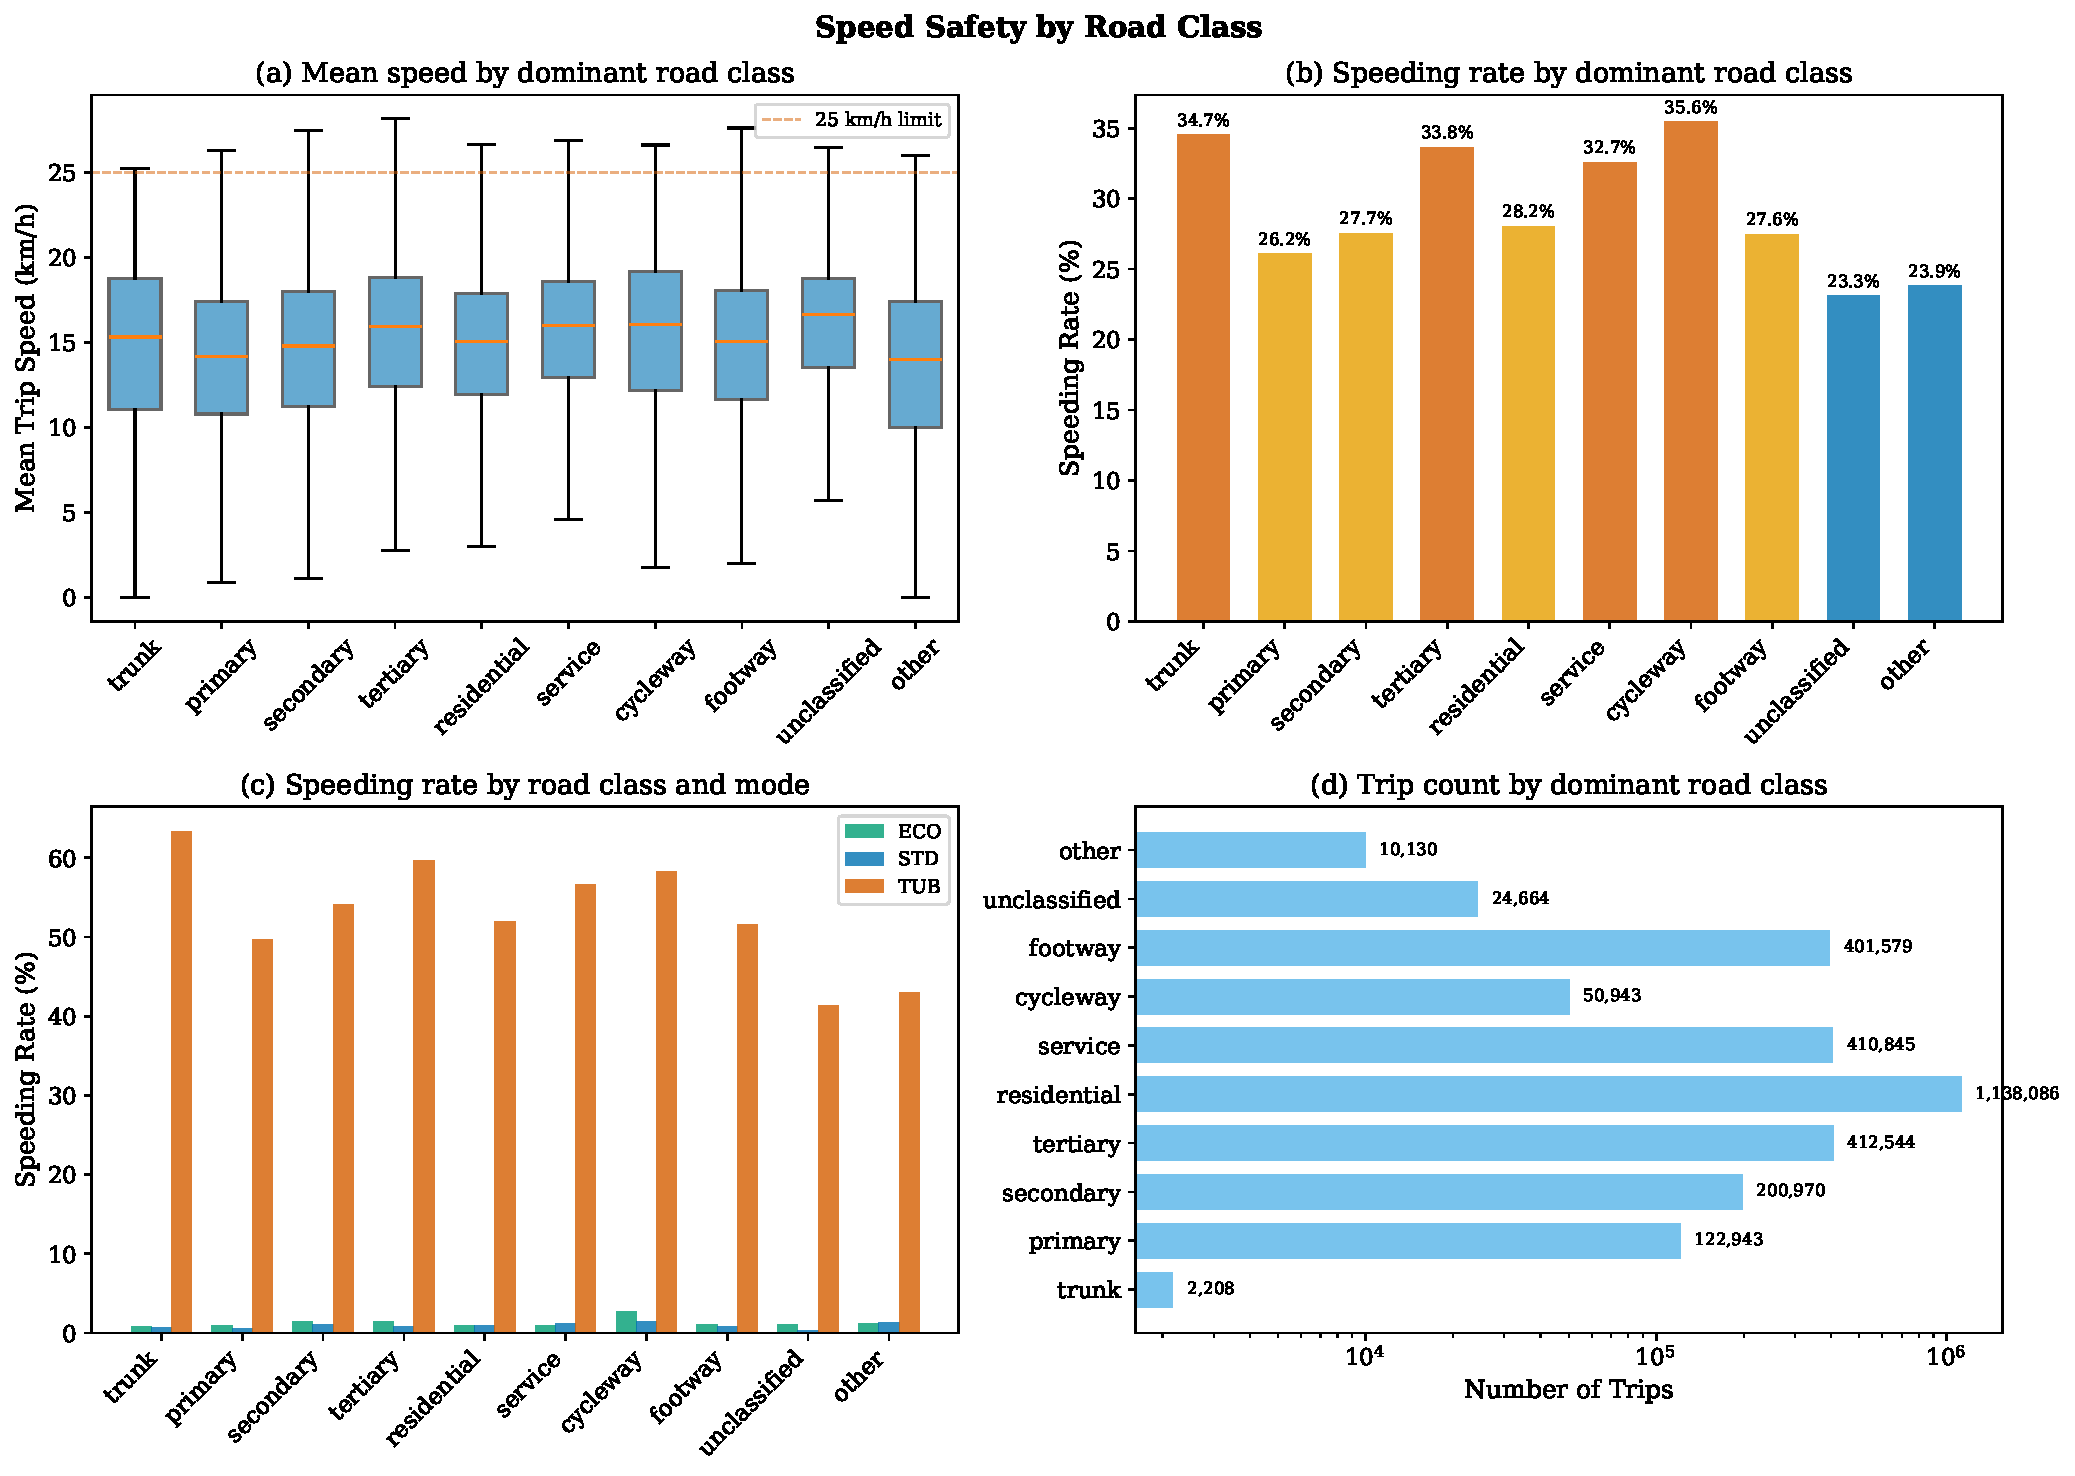
\includegraphics[width=\textwidth]{figures/fig8_speed_by_road_class.pdf}
\caption{Speed safety indicators by road class. Four panels: (a) mean speed box plots by road class, (b) speeding rate bar chart by road class, (c) mode $\times$ road class interaction for speeding rate, and (d) trip count distribution across road classes.}
\label{fig:road_class}
\end{figure}

\subsection{Logistic Regression for Speeding Propensity (Model 1)}
\label{sec:res_logistic}

Table~\ref{tab:logistic} summarizes the key odds ratios from the logistic regression (Model~1), estimated on the full dataset of 2,319,886 scooter-mode trips (pseudo-$R^2 = 0.354$). Figure~\ref{fig:forest_plot} presents the corresponding forest plot.

\begin{table}[htbp]
\centering
\caption{Logistic regression odds ratios for trip-level speeding propensity (Model~1). Reference categories: age $<$20, STD mode, midday, weekday, Seoul.}
\label{tab:logistic}
\footnotesize
\begin{tabular}{lrrrl}
\toprule
\textbf{Variable} & \textbf{OR} & \textbf{95\% CI} & \textbf{$p$-value} \\
\midrule
\multicolumn{4}{l}{\textit{Operating mode (ref: STD)}} \\
\quad TUB & 121.3 & [118.8, 124.0] & $< 0.001$ \\
\quad ECO & 1.17 & [1.10, 1.25] & $< 0.001$ \\
\addlinespace
\multicolumn{4}{l}{\textit{Age group (ref: $<$20)}} \\
\quad 20--24 & 0.87 & [0.87, 0.88] & $< 0.001$ \\
\quad 25--29 & 0.76 & [0.75, 0.77] & $< 0.001$ \\
\quad 30--34 & 0.70 & [0.69, 0.71] & $< 0.001$ \\
\quad 35--39 & 0.74 & [0.72, 0.75] & $< 0.001$ \\
\quad 40--49 & 0.88 & [0.86, 0.89] & $< 0.001$ \\
\quad 50--59 & 0.85 & [0.83, 0.87] & $< 0.001$ \\
\quad 60+ & 0.81 & [0.79, 0.84] & $< 0.001$ \\
\addlinespace
\multicolumn{4}{l}{\textit{Time of day (ref: midday)}} \\
\quad Morning rush & 0.89 & [0.88, 0.91] & $< 0.001$ \\
\quad Afternoon rush & 1.04 & [1.03, 1.06] & $< 0.001$ \\
\quad Evening & 0.79 & [0.78, 0.80] & $< 0.001$ \\
\quad Night & 0.84 & [0.83, 0.85] & $< 0.001$ \\
\addlinespace
\multicolumn{4}{l}{\textit{Day type (ref: weekday)}} \\
\quad Saturday & 1.03 & [1.02, 1.04] & $< 0.001$ \\
\quad Sunday & 0.93 & [0.92, 0.94] & $< 0.001$ \\
\addlinespace
\multicolumn{4}{l}{\textit{Province (ref: Seoul; selected)}} \\
\quad Chungnam & 2.79 & [2.74, 2.83] & $< 0.001$ \\
\quad Gyeongbuk & 2.72 & [2.67, 2.78] & $< 0.001$ \\
\quad Gangwon & 2.58 & [2.52, 2.65] & $< 0.001$ \\
\quad Daegu & 2.23 & [2.18, 2.29] & $< 0.001$ \\
\quad Chungbuk & 2.16 & [2.10, 2.22] & $< 0.001$ \\
\quad Gyeonggi & 1.59 & [1.58, 1.61] & $< 0.001$ \\
\quad Daejeon & 1.48 & [1.46, 1.51] & $< 0.001$ \\
\midrule
$N$ & \multicolumn{3}{l}{2,319,886 trips} \\
Pseudo-$R^2$ & \multicolumn{3}{l}{0.354} \\
\bottomrule
\end{tabular}
\end{table}

TUB mode dominates: riders have 121 times the odds of speeding versus STD (OR $= 121.3$, 95\% CI: [118.8, 124.0]). All age groups show lower odds than the under-20 reference, with the 30--34 group most protective (OR $= 0.70$). The age gradient is non-monotonic, partially recovering for 40+ groups. After controlling for mode, speeding odds are \textit{lower} during evening (OR $= 0.79$) and night (OR $= 0.84$) than midday---reversing the raw descriptive patterns, which reflect confounding by TUB mode composition among late-night riders. Substantial provincial variation persists (Chungnam OR $= 2.79$ vs. Seoul).

The GEE specification (Figure~\ref{fig:gee_forest}) produces consistent results: TUB OR $= 109$ [100, 118], modestly attenuated by accounting for within-user dependence but qualitatively identical.

\begin{figure}[htbp]
\centering
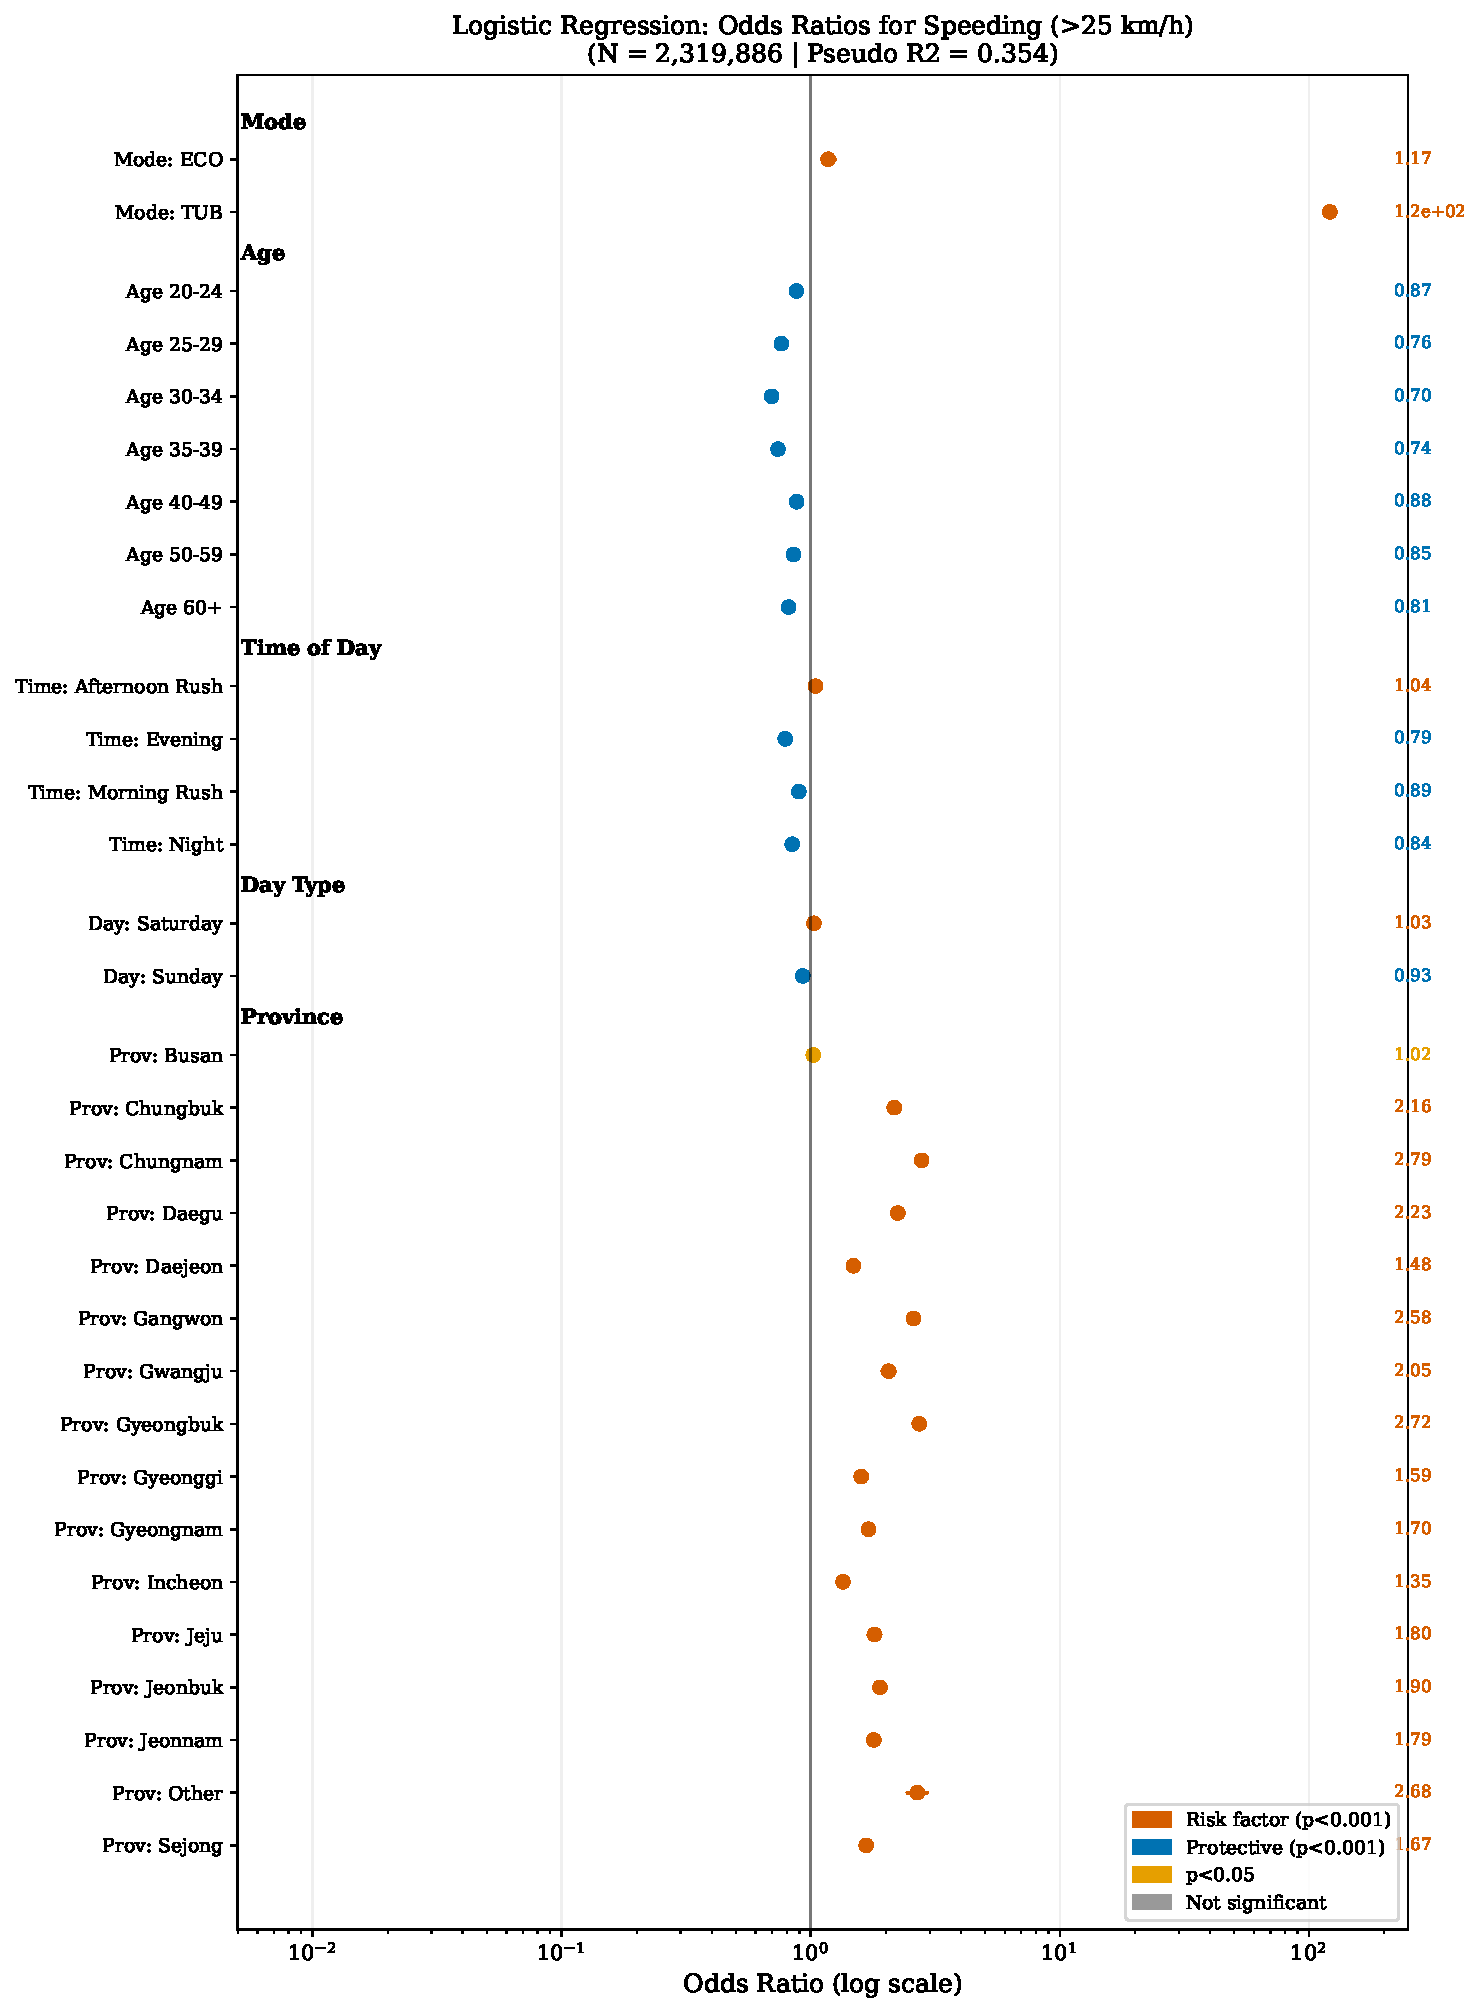
\includegraphics[width=0.85\textwidth]{figures/fig9_logistic_OR.pdf}
\caption{Forest plot of odds ratios from the logistic regression (Model~1, full dataset). Points indicate estimated ORs; horizontal bars indicate 95\% confidence intervals. The vertical dashed line at OR $= 1$ indicates the null effect. Variables are grouped by category and color-coded by significance level.}
\label{fig:forest_plot}
\end{figure}

\begin{figure}[htbp]
\centering
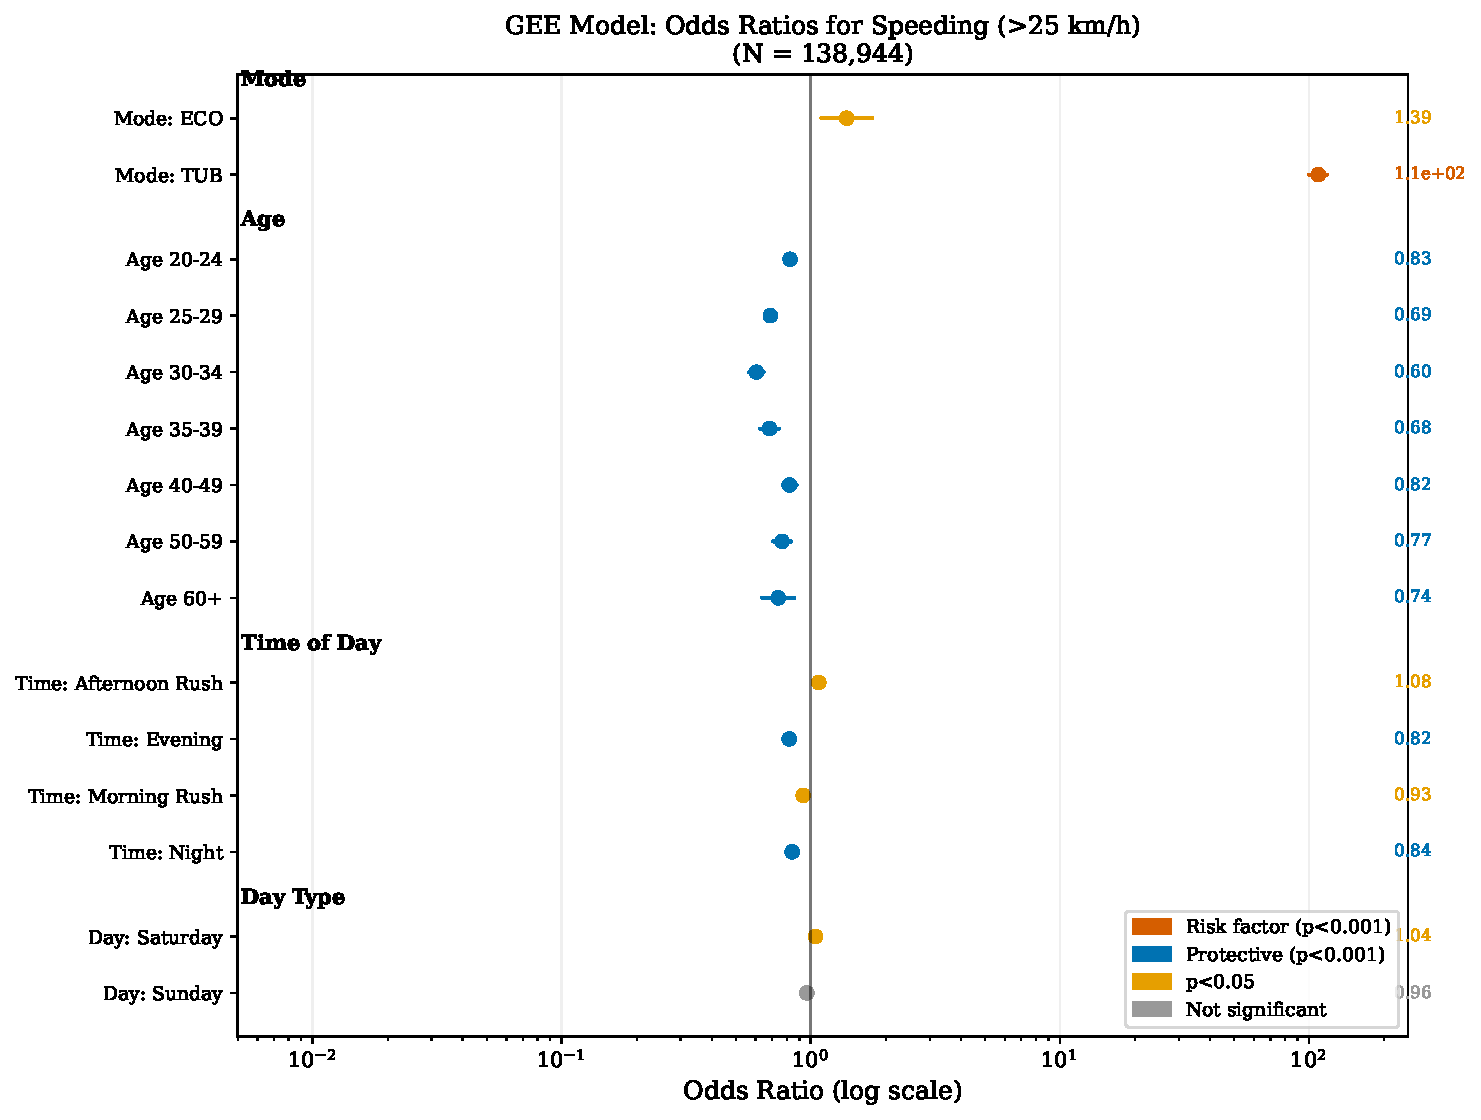
\includegraphics[width=0.85\textwidth]{figures/fig10_gee_OR.pdf}
\caption{Forest plot of odds ratios from the GEE logistic regression (Model~1, 200,000-trip subsample with exchangeable working correlation). Format follows Figure~\ref{fig:forest_plot}.}
\label{fig:gee_forest}
\end{figure}

\subsection{Mixed-Effects Linear Model for Mean Speed (Model 2)}
\label{sec:res_mixed}

The mixed-effects model (100,000 trips, 67,799 users) yields ICC $= 0.271$: 27.1\% of speed variance is between-user. TUB mode increases mean speed by 2.2~km/h ($p < 0.001$), ECO decreases it by 2.6~km/h. Service roads are 0.65~km/h faster than residential; footways 0.81~km/h slower. Counter-intuitively, $\text{frac\_major\_road}$ has a negative coefficient ($-2.2$~km/h), suggesting congestion constrains e-scooter speeds on major roads.

\subsection{Two-Part Hurdle Model for Speeding Intensity (Model 3)}
\label{sec:res_hurdle}

The hurdle model (Part~1 pseudo-$R^2 = 0.382$) separates occurrence from intensity. In Part~1 (occurrence), TUB mode dominates (OR $= 126.6$), cycling infrastructure is protective (OR $= 0.71$), and major roads reduce speeding probability (OR $= 0.62$). In Part~2 (intensity, $n = 59{,}144$ speeding trips), cycling infrastructure paradoxically \textit{increases} intensity ($\beta = 1.14$, $p = 0.009$): dedicated paths reduce the probability of speeding but enable sustained high speeds when it occurs. Major roads remain protective in Part~2 ($\beta = -0.26$), consistent with congestion effects.

\subsection{Rider Speed Behavior Typology (Model 4)}
\label{sec:res_typology}

The GMM analysis of 198,821 users with at least 3 trips identifies four distinct rider typologies (Figure~\ref{fig:gmm_radar}):

\begin{enumerate}
    \item \textbf{Safe Riders} (40.3\%, $n = 80{,}052$): Zero speeding propensity, moderate mean speed (13.1~km/h), low speed variability (CV $= 0.53$), and moderate cruise fraction. These riders never exceed 25~km/h during any recorded trip.

    \item \textbf{Moderate-Risk Riders} (25.9\%, $n = 51{,}491$): Moderate speeding propensity (0.30), mean max speed of 23.6~km/h (approaching but below the limit), moderate harsh event rates. These riders occasionally speed but not as a persistent pattern.

    \item \textbf{Habitual Speeders} (26.3\%, $n = 52{,}223$): High speeding propensity (0.59), highest mean speed (17.9~km/h) and mean max speed (25.1~km/h), with the highest speeding rate (0.12). A majority of trips by these users involve at least one speeding event.

    \item \textbf{Stop-and-Go Riders} (7.6\%, $n = 15{,}055$): Moderate speeding propensity (0.34) but the highest speed variability (CV $= 0.65$), highest zero-speed fraction (0.27), and highest harsh acceleration/deceleration propensity. These riders exhibit erratic speed profiles with frequent stops and starts.
\end{enumerate}

Multinomial logistic regression predicting class membership (reference: Safe Rider, pseudo-$R^2 = 0.297$) reveals that TUB mode usage is overwhelmingly the strongest predictor of belonging to higher-risk classes (Figure~\ref{fig:multinomial}, Appendix). The relative risk ratio (RRR) for TUB mode is 11.8 for the Habitual Speeder class ($p < 0.001$) and 1.76 for the Moderate-Risk class ($p < 0.001$). Conversely, ECO mode usage is strongly protective (RRR $= 0.06$ for Habitual Speeder, $p < 0.001$). Age effects are consistent with the trip-level models: younger riders are more likely to belong to the Habitual Speeder class, with the 30--34 age group least likely. Geographic effects are also significant: riders in Chungnam, Gyeongnam, and Daejeon provinces are more likely to belong to higher-risk classes compared to Seoul riders.

\begin{figure}[htbp]
\centering
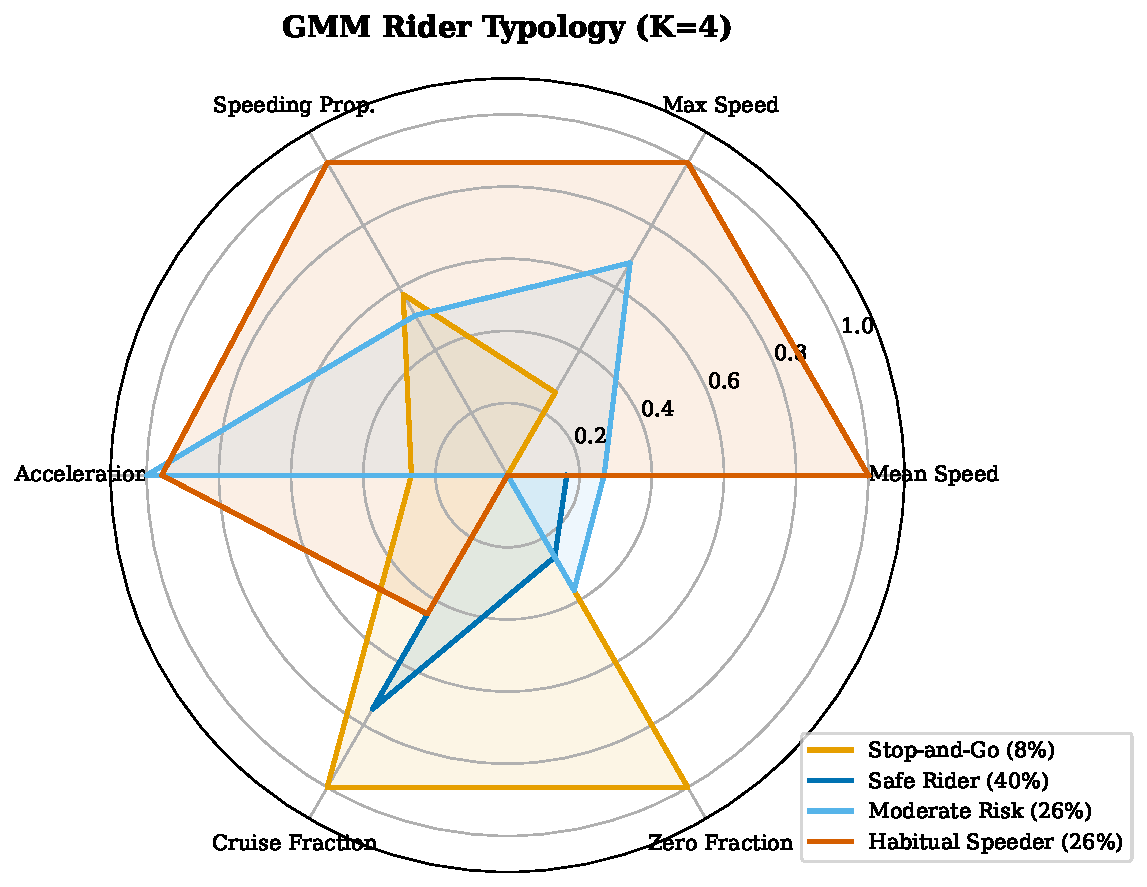
\includegraphics[width=0.85\textwidth]{figures/fig11_rider_typology_radar.pdf}
\caption{Radar (spider) plots of normalized speed behavior features for the four GMM-identified rider typologies. Each axis represents a standardized speed indicator; the polygonal area reflects the overall behavioral profile. Safe Riders (40\%), Moderate-Risk (26\%), Habitual Speeders (26\%), and Stop-and-Go (8\%).}
\label{fig:gmm_radar}
\end{figure}

\subsection{Natural Experiment: Speed Governor Effectiveness}
\label{sec:res_governor}

Table~\ref{tab:mode_comparison} presents the within-subject comparison of TUB versus ECO mode among 12,046 users who used both modes during the observation period. The speed governor produces large and highly significant reductions across all speed metrics. Mean speed decreases from 15.4~km/h (TUB) to 11.7~km/h (ECO), a reduction of 3.7~km/h (24\%, Cohen's $d = 1.00$). Maximum speed decreases from 24.6~km/h to 16.9~km/h, a reduction of 7.7~km/h (31\%, Cohen's $d = 2.17$). The speeding rate drops from 7.4\% to 0.38\%, a 20-fold reduction ($p < 0.001$ for both paired $t$-test and Wilcoxon signed-rank test). Figure~\ref{fig:tub_eco} visualizes these within-subject differences.

\begin{table}[htbp]
\centering
\caption{Within-subject comparison of TUB vs.\ ECO mode ($n = 12{,}046$ paired users).}
\label{tab:mode_comparison}
\small
\begin{tabular}{lrrrrl}
\toprule
\textbf{Metric} & \textbf{TUB} & \textbf{ECO} & \textbf{Diff.} & \textbf{Cohen's $d$} & \textbf{$p$-value} \\
\midrule
Mean speed (km/h) & 15.4 & 11.7 & $-3.7$ & 1.00 & $< 0.001$ \\
Max speed (km/h) & 24.6 & 16.9 & $-7.7$ & 2.17 & $< 0.001$ \\
P85 speed (km/h) & 22.4 & 15.8 & $-6.7$ & 1.77 & $< 0.001$ \\
Speeding rate (\%) & 7.4 & 0.38 & $-7.0$ & 0.79 & $< 0.001$ \\
Speed CV & 0.54 & 0.48 & $-0.06$ & 0.22 & $< 0.001$ \\
\bottomrule
\end{tabular}
\end{table}

Speed CV shows a small effect ($d = 0.22$) compared to speed-level effects ($d = 1.0$--$2.2$), indicating that the governor compresses the speed distribution downward without substantially altering riding dynamics.

\begin{figure}[htbp]
\centering
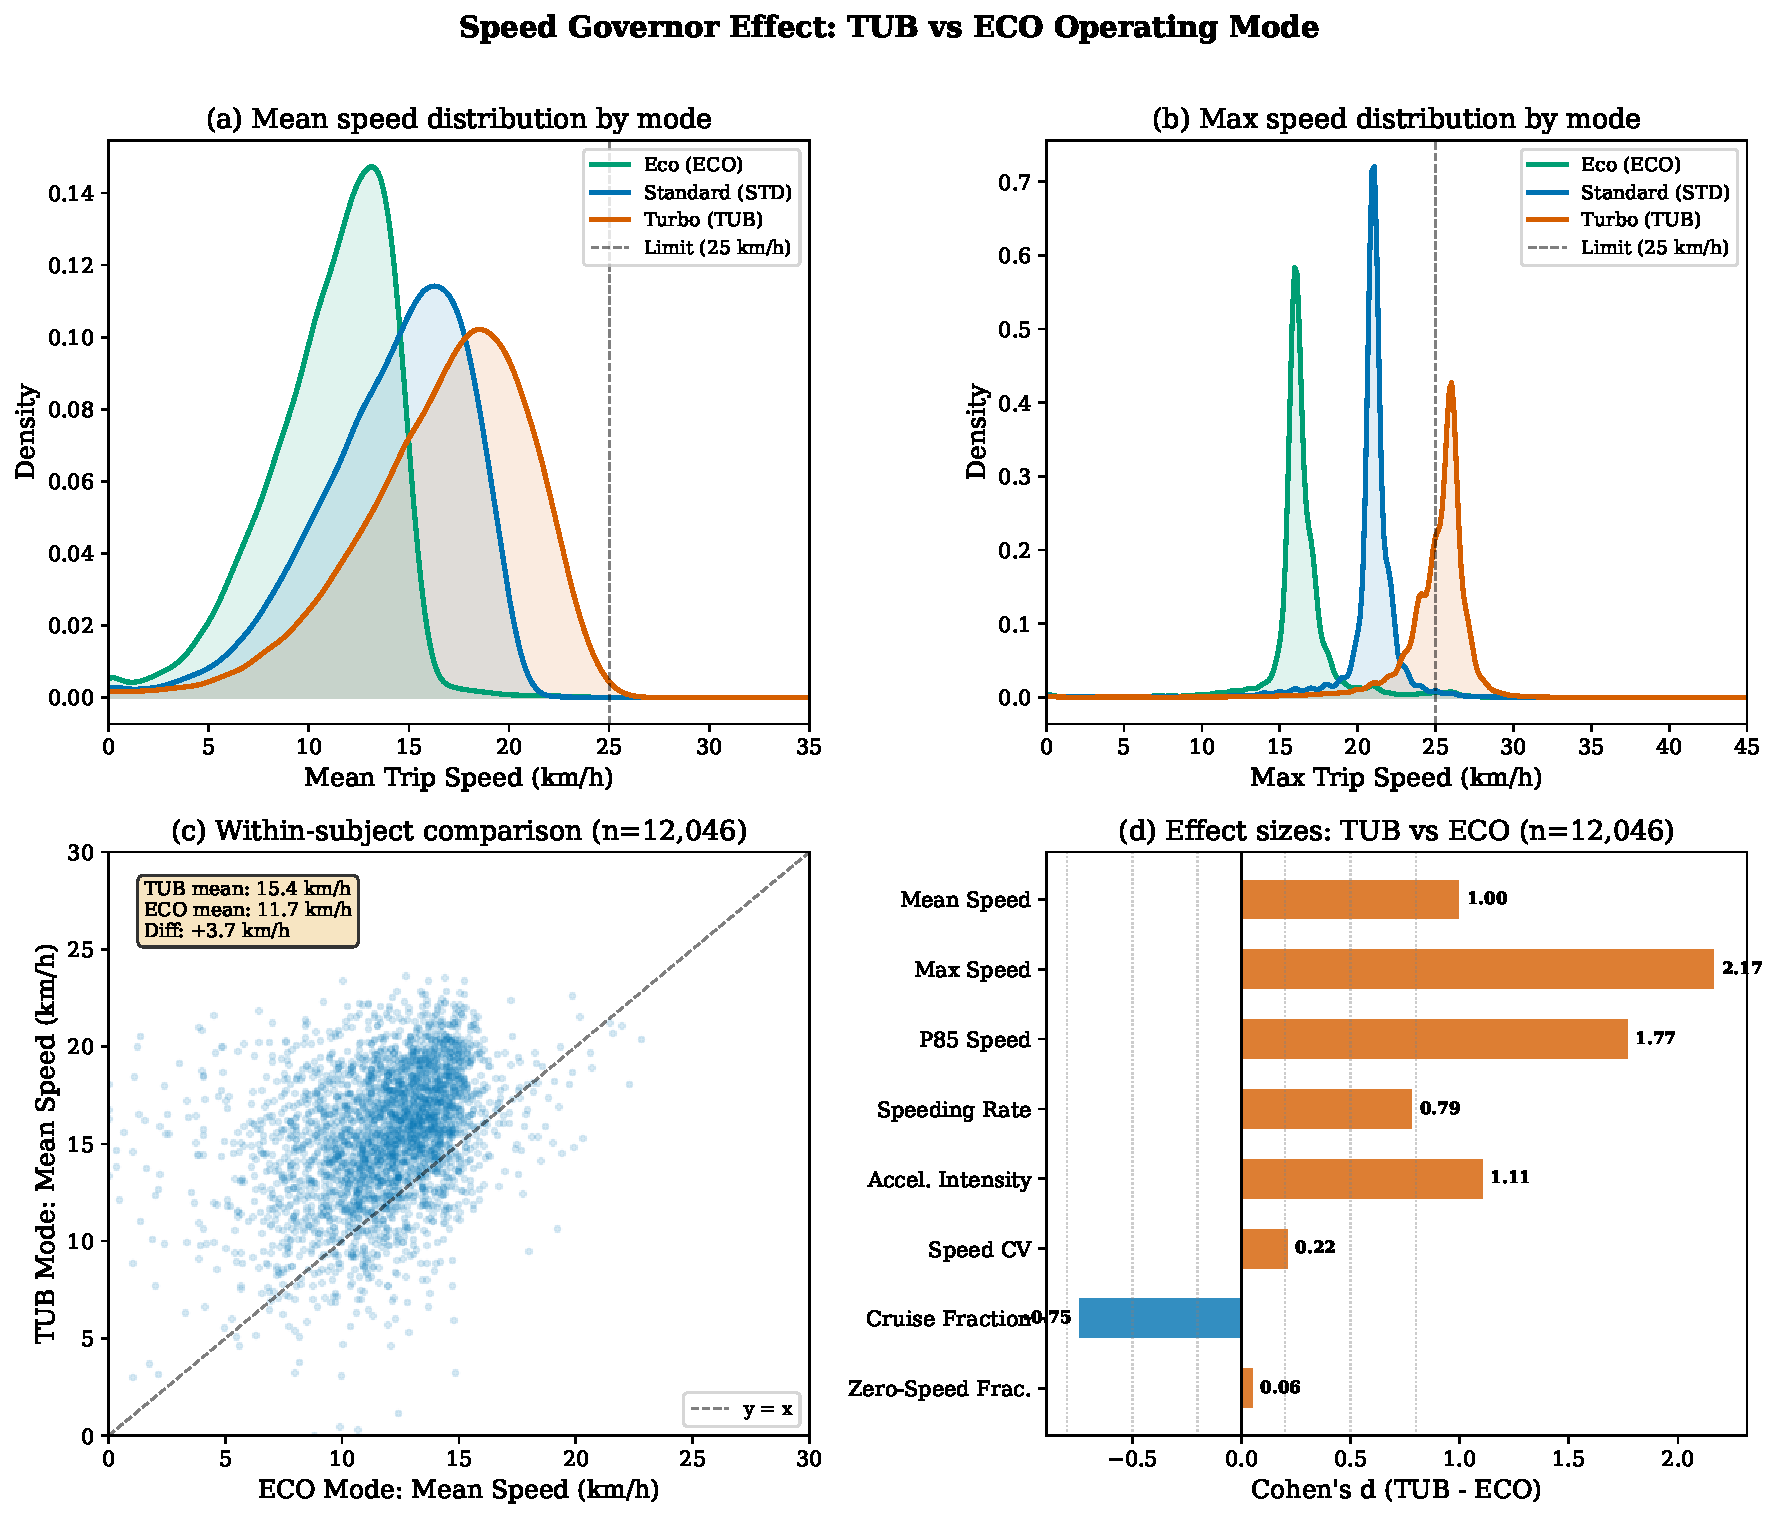
\includegraphics[width=\textwidth]{figures/fig12_tub_vs_eco.pdf}
\caption{TUB vs.\ ECO mode comparison among 12,046 users who used both modes. Four panels: (a) mean speed density distributions, (b) maximum speed density distributions, (c) within-subject paired scatter plot (each point is one user), and (d) effect size bar chart with Cohen's $d$ for each speed metric.}
\label{fig:tub_eco}
\end{figure}

\subsection{Robustness Checks}
\label{sec:res_robust}

All robustness checks confirm core findings (see Figures~\ref{fig:robust_threshold}, \ref{fig:robust_subsample}, and~\ref{fig:robust_city} in Appendix). Threshold sensitivity: at 20~km/h, 87.1\% of trips involve speeding (TUB OR $= 4.0$); at 25~km/h, 30.1\% (OR $= 121$); at 30~km/h, 0.2\%. Subsampling: TUB OR CV $= 1.2\%$ across five 200K-trip subsamples. City-specific: TUB OR ranges from 70 (Suwon) to 207 (Daejeon); direction and significance universal across all five cities. OLS coefficient estimates are shown in Figure~\ref{fig:ols_coefficients} (Appendix).

\subsection{Extension: Rider Experience and Speeding}
\label{sec:res_experience}

Speeding increases monotonically with experience: from 3.8\% on a rider's first trip to 28.0\% after 500+ trips (Table~\ref{tab:experience}).

\begin{table}[htbp]
\centering
\caption{Speeding prevalence by rider experience (trip rank).}
\label{tab:experience}
\small
\begin{tabular}{lrrl}
\toprule
\textbf{Experience bin} & \textbf{Trips} & \textbf{Users} & \textbf{Speeding rate} \\
\midrule
1st trip & 1,816,911 & 1,816,911 & 3.8\% \\
2--5 trips & 4,497,120 & 1,365,628 & 5.4\% \\
6--20 trips & 9,184,824 & 866,253 & 8.5\% \\
21--50 trips & 9,193,834 & 436,746 & 12.8\% \\
51--100 trips & 7,397,225 & 214,458 & 17.2\% \\
101--500 trips & 10,673,925 & 100,793 & 23.8\% \\
500+ trips & 1,356,904 & 5,516 & 28.0\% \\
\bottomrule
\end{tabular}
\end{table}

The GEE model (Model~6; 50,000 users, 1.19M trips) confirms: each doubling of trip rank increases speeding odds by 17.8\% (OR $= 1.178$, 95\% CI: [1.156, 1.200], $p < 10^{-66}$), with no quadratic effect ($p = 0.44$). Newcomers speed at 15.6\% versus 26.7\% for established riders (Cohen's $d = 0.256$).

Critically, this effect is mediated by \textit{mode adoption}: TUB usage rises from 11.5\% at trip~1 to 47.8\% by trip~50 (Figure~\ref{fig:mode_adoption}, Appendix). Within operating modes, the newcomer--established difference nearly vanishes (STD: 1.0\% vs. 0.8\%; TUB: 49.6\% vs. 50.7\%; Figure~\ref{fig:newcomer_established}, Appendix). Riders do not learn to ride faster---they increasingly select TUB mode. Detailed experience curves (Figure~\ref{fig:experience_curve}), newcomer trajectories (Figure~\ref{fig:newcomer_trajectory}), and usage category breakdowns (Figure~\ref{fig:usage_category}) are provided in the Appendix.

\subsection{Extension: Trip Distance and Road Composition}
\label{sec:res_distance}

Speeding increases monotonically with distance: 13.9\% (shortest decile, 149~m) to 54.2\% (longest, 2,168~m; Figure~\ref{fig:distance_curve}, Appendix). The spline logistic regression (Model~7; pseudo-$R^2 = 0.387$; Figure~\ref{fig:distance_spline}, Appendix) captures the non-linear relationship. Road composition ORs reveal a congestion interpretation: service (2.74) and tertiary (2.05) roads enable speeding, while primary (0.13) and secondary (0.20) roads---with higher traffic volumes---are strongly protective (Figure~\ref{fig:road_or}, Appendix). Riders slow down by 1.5~km/h in the second half of trips on average (Figure~\ref{fig:speed_drift}, Appendix). Road class $\times$ distance interactions are shown in Figure~\ref{fig:distance_road_heatmap} (Appendix).

\subsection{Extension: Trajectory Curvature and Speeding Risk}
\label{sec:res_curvature}

Higher curvature is associated with lower speeding: OR $= 0.716$ [0.699, 0.732]. Speeding rates decrease from 41.0\% (straightest quintile) to 16.8\% (curviest; Figure~\ref{fig:curvature_rate}, Appendix)---physically intuitive, as riders cannot sustain speeds through turns. However, a risk paradox emerges: the composite risk score (speed excess $\times$ curvature) is 5$\times$ higher when speeding occurs on curvy roads (Figure~\ref{fig:curvature_risk}, Appendix). This implies a dual enforcement strategy: target straight segments (high prevalence) and curvy segments (high consequences). Road class interactions with curvature are shown in Figure~\ref{fig:curvature_roadclass} (Appendix).

\subsection{Extension: SHAP Feature Importance}
\label{sec:res_shap}

The LightGBM model (AUC $= 0.905$, F1 $= 0.739$) confirms the parametric findings via SHAP (Figures~\ref{fig:shap_beeswarm}--\ref{fig:shap_dependence}, Appendix). TUB mode dominates (mean SHAP $= 2.33$, 3.6$\times$ the next feature; Figure~\ref{fig:shap_bar}, Appendix), followed by log-distance (0.64), mean acceleration (0.50), cruise fraction (0.26), and speed CV (0.25). SHAP dependence plots reveal non-linearities---distance effect saturation, threshold-like acceleration effects---that the logistic specification does not capture, strengthening confidence in the core findings through concordance between parametric and non-parametric approaches.

\subsection{Extension: Causal Effect of Speed Governor Restriction (Model 9)}
\label{sec:res_did}

The December 2023 TUB ban (54.6\% $\rightarrow$ 1.4\% system-wide) provides a natural experiment. Pre-ban TUB adoption varied across cities (32--70\%), enabling identification via treatment intensity variation (Figure~\ref{fig:did_mode_trends}).

\begin{figure}[htbp]
\centering
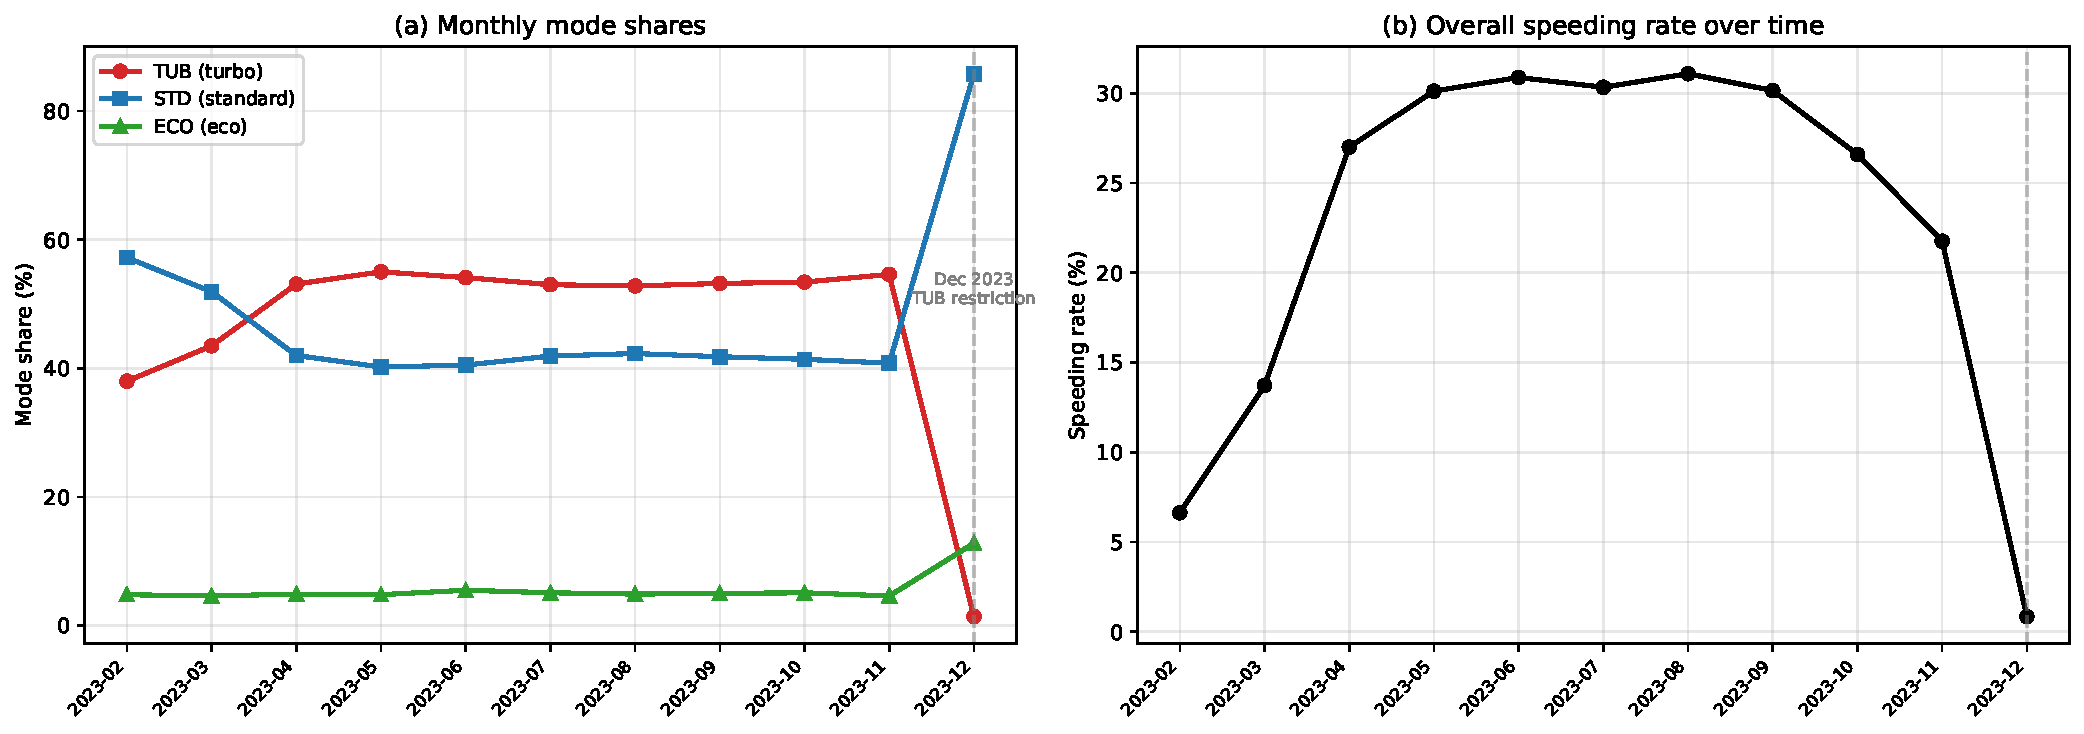
\includegraphics[width=\textwidth]{figures/fig_did_mode_trends.pdf}
\caption{Monthly mode share and overall speeding rate across all cities (February--December 2023). The vertical dashed line marks December 2023, when TUB mode was effectively banned. TUB share (red) collapses from 54.6\% to 1.4\%, while the overall speeding rate drops from approximately 28\% to approximately 1\%.}
\label{fig:did_mode_trends}
\end{figure}

\subsubsection{TWFE DiD Estimates}

The TWFE coefficient (Table~\ref{tab:did_results}) is $\hat{\beta} = -0.568$ (cluster SE $= 0.077$, $p < 10^{-13}$): a city with 50\% pre-ban TUB share experienced a 28.4~pp speeding reduction. Cluster-robust and HC1 SEs are nearly identical (ratio $= 1.03$), indicating negligible serial correlation.

\begin{table}[htbp]
\centering
\caption{Difference-in-Differences estimates of TUB mode restriction on speeding. All estimates normalized to the effect per 10 percentage point change in TUB share.}
\label{tab:did_results}
\small
\begin{tabular}{lrrrl}
\toprule
\textbf{Model} & \textbf{Effect per 10pp} & \textbf{SE} & \textbf{95\% CI} & \textbf{$p$-value} \\
\midrule
Cross-sectional OLS & $-4.9$~pp & 0.64 & [$-6.1$, $-3.6$] & $< 0.001$ \\
TWFE DiD (cluster SEs) & $-5.7$~pp & 0.77 & [$-7.2$, $-4.2$] & $< 0.001$ \\
Event study (Dec coef) & $-4.8$~pp & 0.67 & [$-6.1$, $-3.5$] & $< 0.001$ \\
Dose-response (bootstrap) & $+5.0$~pp & --- & [$+4.1$, $+7.4$] & $< 0.001$ \\
\bottomrule
\end{tabular}
\begin{flushleft}
\footnotesize \textit{Note:} Cross-sectional and TWFE effects are per 10pp of pre-ban TUB share (higher share $\rightarrow$ larger speeding reduction). Dose-response effect is per 10pp of TUB share reduction (larger reduction $\rightarrow$ larger speeding reduction). All models weighted by $\sqrt{N_{\text{trips}}}$; TWFE includes city and month fixed effects. Dose-response CI is bootstrapped (10,000 replications). Panel: 53 cities, 563 observations.
\end{flushleft}
\end{table}

\subsubsection{Event Study and Pre-trends}

The event study (Figure~\ref{fig:did_event_study_v2}a) shows the December coefficient ($\hat{\delta}_1 = -0.483$) is substantially larger than any pre-period coefficient ($+0.11$ to $+0.22$). The joint $F$-test rejects parallel trends ($F = 20.0$, $p < 0.001$), but three considerations support causal interpretation \citep{roth2022pretest}. First, the pre-trend is \textit{positive} (conservative direction): cities with higher TUB adoption had increasing speeding, so the December reversal underestimates the true effect. Second, the de-trended specification yields a near-identical coefficient ($\hat{\delta}_1 = -0.481$; Figure~\ref{fig:did_event_study_v2}b), with the linear trend itself non-significant ($p = 0.74$). Third, the treatment effect is 3--4$\times$ larger than the largest stable pre-period coefficient.

\begin{figure}[htbp]
\centering
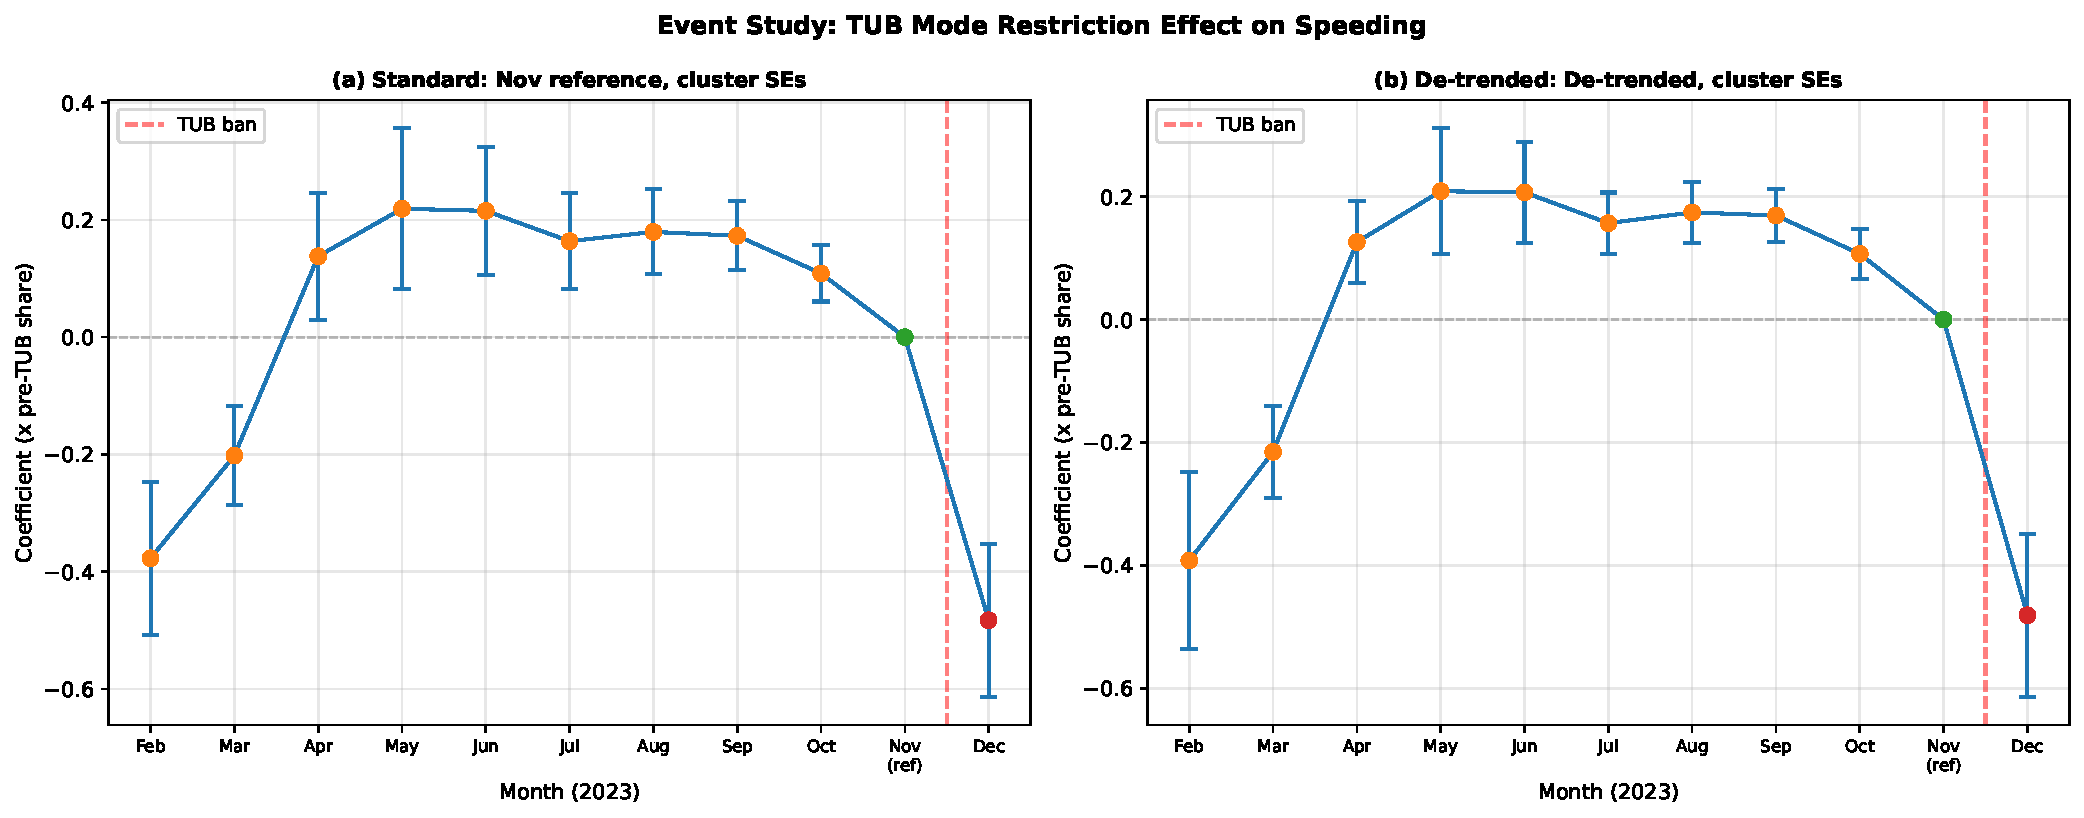
\includegraphics[width=\textwidth]{figures/fig_did_event_study_v2.pdf}
\caption{Event study: interaction coefficients between month indicators and pre-ban TUB share, with November 2023 as reference ($k = 0$). Cluster-robust 95\% confidence intervals. (a) Standard specification. (b) De-trended specification absorbing a linear time-by-treatment interaction. The December coefficient (red) represents the treatment effect; pre-period coefficients (orange if significant, blue if not) test for differential pre-trends.}
\label{fig:did_event_study_v2}
\end{figure}

\subsubsection{Dose-Response and Robustness}

The dose-response confirms: each 10~pp TUB reduction produces a 5.0~pp speeding reduction ($r = 0.754$, bootstrap CI: [0.56, 0.87]; Figure~\ref{fig:did_dose_response}). The placebo test (September as fictitious treatment) yields $\hat{\beta} = -0.015$, $p = 0.56$---no spurious effects. Heterogeneity analysis shows consistent effects across all city-size quartiles (20--25~pp, all $p < 0.001$; Figure~\ref{fig:did_robustness}).

\begin{figure}[htbp]
\centering
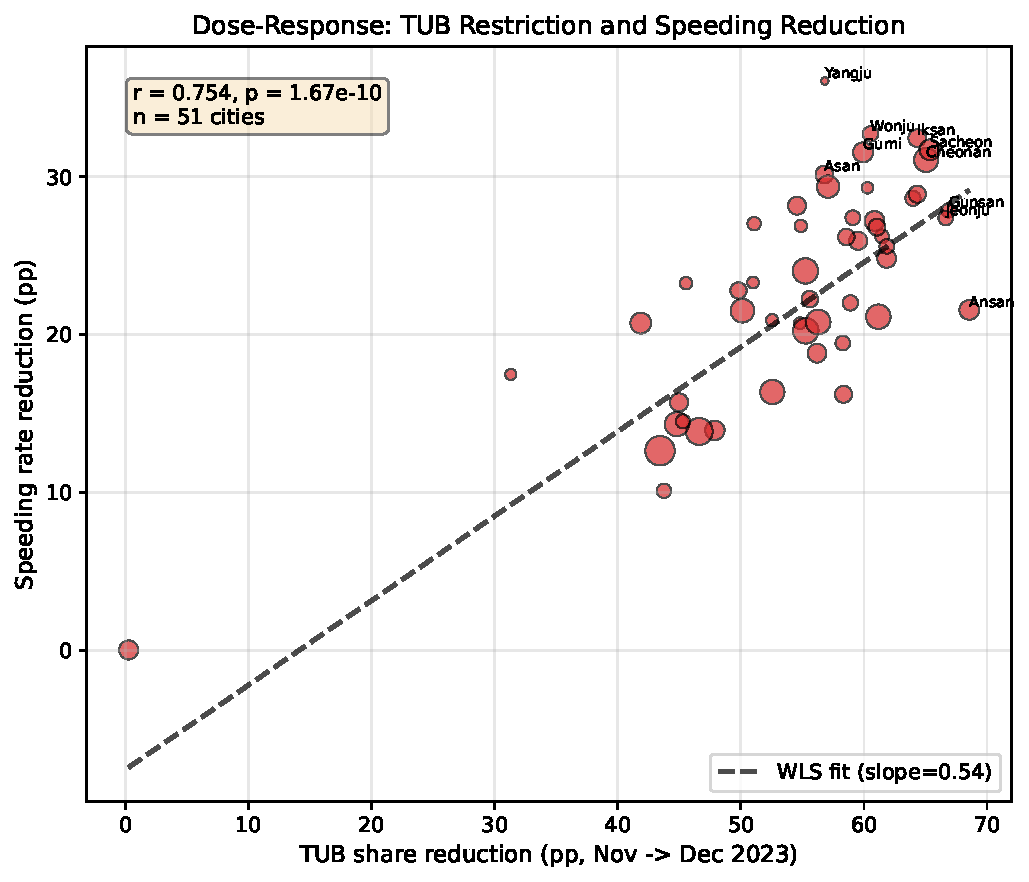
\includegraphics[width=0.8\textwidth]{figures/fig_did_dose_response.pdf}
\caption{Dose-response: city-level TUB share reduction versus speeding reduction. Dashed line: WLS fit. $r = 0.754$ [0.56, 0.87], $n = 51$ cities.}
\label{fig:did_dose_response}
\end{figure}

\begin{figure}[htbp]
\centering
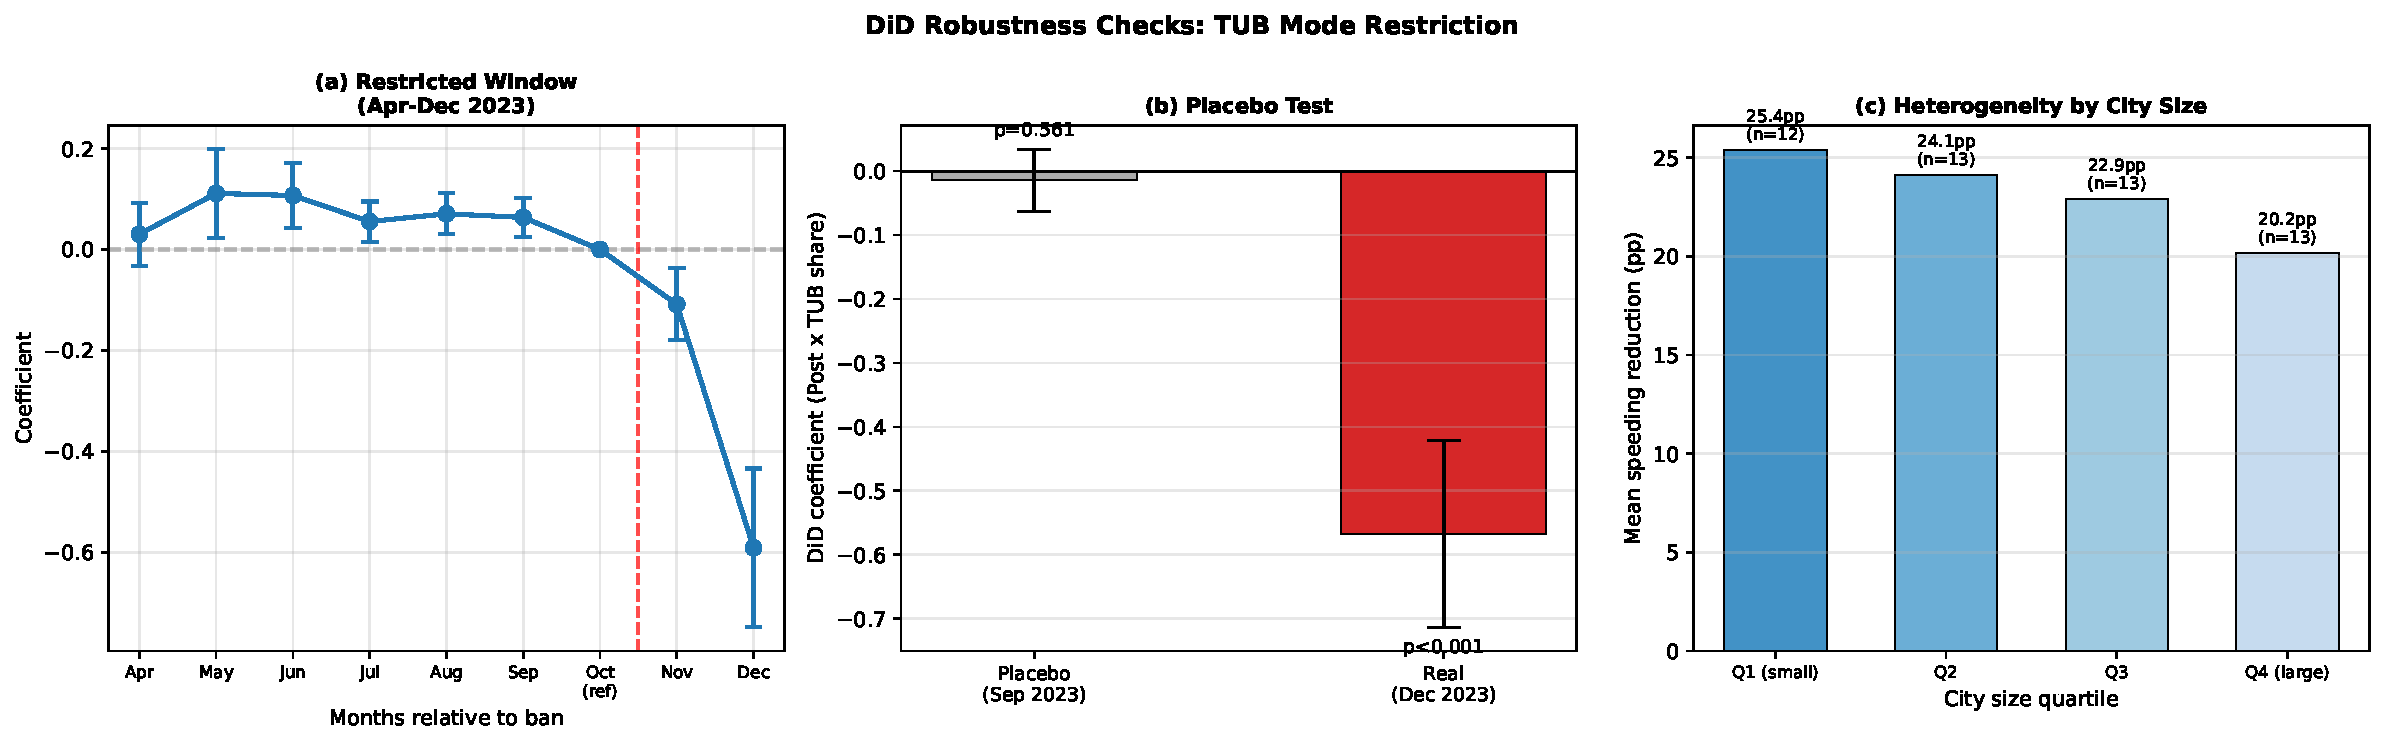
\includegraphics[width=\textwidth]{figures/fig_did_robustness.pdf}
\caption{DiD robustness: (a) restricted event window, (b) placebo test ($p = 0.56$), (c) heterogeneity by city size (20--25~pp, all $p < 0.001$).}
\label{fig:did_robustness}
\end{figure}

Together, the consistency across four estimation strategies, null placebo test, and treatment magnitude (3--4$\times$ pre-period coefficients) support causal interpretation. These population-level estimates complement the within-subject analysis (Section~\ref{sec:res_governor}). A user-level mode-switcher analysis confirms that the aggregate STD/ECO speed increase reflects a composition effect (faster riders joining the pool) rather than risk compensation (within-user DiD: $+0.20$~km/h, $d = 0.069$; placebo DiD: $-0.08$~km/h; Figures~\ref{fig:mode_switcher}--\ref{fig:mode_switcher_placebo}, Appendix). Additional DiD visualizations---the December transition scatter plot (Figure~\ref{fig:did_dec_transition}), individual city trend lines (Figure~\ref{fig:did_city_trends}), parallel trends diagnostics (Figure~\ref{fig:did_parallel_trends}), and a summary coefficient comparison (Figure~\ref{fig:did_summary})---are provided in the Appendix.
